\documentclass[a4paper,twoside]{report}
% Enable UTF-8 text
\usepackage[utf8]{inputenc} % enable UTF-8 text

% Adds bibliography to table of contents
\usepackage[nottoc]{tocbibind}

% Automatically collect used acronyms
\usepackage[printonlyused,withpage]{acronym}
%
% Automatically add acronyms to index, see
% http://tex.stackexchange.com/questions/22570/automatically-index-acronyms
%
% I have turned these off temporarily, because it gave pretty strange
% results.
%
%   \let\oldac\ac
%   \renewcommand*{\ac}[1]{\oldac{#1}\index{#1}}
%
% (Could also use the nomencl package here, which supports it)

% Use newlines in paragraph instead of indentation
\usepackage{parskip}

% Adds the TODO package
\usepackage[backgroundcolor=white,linecolor=red,bordercolor=red]{todonotes}

% Build index, using the new imakeidx in TeX Live, see
% http://tex.blogoverflow.com/2012/09/dont-forget-to-run-makeindex/
\usepackage{imakeidx}
\makeindex

% Uncomment this if you want to show all \index{} locations in the document
% in the margins (good for proofreading)
%\usepackage{showidx}

% Hyperlinks, clickable references
% Hidelinks turns off colored box on some PDF viewers
\usepackage[hidelinks]{hyperref}

% On Mac OSX, in ViM, when I type ALT+SHIFT+SPACE (often typed accidentally
% after writing {\some-command ...}, then LaTeX may give me the error
% "Unicode char \u8:  not set up for use with LaTeX.".  This character
% in UTF-8 actually means what the tilde (~) means in LaTeX, but *I*
% usually mean just a space.  This command replaces those with a
% normal space:
\DeclareUnicodeCharacter{00A0}{ }
% If I really want the tilde-behaviour, I can use the command
%\DeclareUnicodeCharacter{00A0}{~}
%
% The above solution was taken from:
% http://tex.stackexchange.com/questions/83440/inputenc-error-unicode-char-u8-not-set-up-for-use-with-latex

% Package for writing algorithms
\usepackage{algorithmicx}
\usepackage{algorithm}
\usepackage[noend]{algpseudocode} % noend -> no "end if" etc.

% Custom \On ... \EndOn block
\algnewcommand\algorithmicon{\textbf{on}}
\algnewcommand\algorithmicfrom{\textbf{from}}
\algblockdefx[ON]{On}{EndOn}[2]
  {\algorithmicon\ #1\ \algorithmicfrom\ #2\ \algorithmicdo}
  {\algorithmicend\ \algorithmicon}
%
% Blank end of block when using [noend] option
\makeatletter
\ifthenelse{\equal{\ALG@noend}{t}}%
  {\algtext*{EndOn}}
  {}%
\makeatother

% Custom \ForIn ... \EndForIn block
\algnewcommand\algorithmicforin{\textbf{for}}
\algnewcommand\algorithmicin{\textbf{in}}
\algblockdefx[FORIN]{ForIn}{EndForIn}[2]
  {\algorithmicforin\ #1\ \algorithmicin\ #2\ \algorithmicdo}
  {\algorithmicend\ \algorithmicforin}
%
% Blank end of block when using [noend] option
\makeatletter
\ifthenelse{\equal{\ALG@noend}{t}}%
  {\algtext*{EndForIn}}
  {}%
\makeatother

% A sendto command
\newcommand{\SendTo}[2]
  {\textbf{send}\ #1\ \textbf{to}\ #2}

\usepackage{amsmath} % for \text{}

% Better verbatim package
\usepackage{fancyvrb}

% For drawing
\usepackage{tikz}

% Above/below refs
\usepackage{varioref}

% Cells spanning vertically
\usepackage{multirow}

% For program listings
\usepackage{listings}
% Make program listings look like verbatim:
% See http://tex.stackexchange.com/questions/172702/how-can-i-make-lstlisting-look-exactly-like-verbatim?noredirect=1#172704
\lstset{
  basicstyle=\ttfamily,
  columns=fullflexible,
  keepspaces=true,
}

\usetikzlibrary{chains, scopes}

% Figures side-by-side
\usepackage{subcaption}

% Used in figures
\definecolor{verylight}{gray}{0.92}

% Hein's space time package for network flows
\usepackage{local-packages/spacetime}

% Nice units
\usepackage{SIunits}
\newcommand\ms[1]{#1~\milli\second}


% If statements ...
\usepackage{ifthen}

% Colors in tables
\usepackage{array} % to control cellspacing, see http://tex.stackexchange.com/questions/98110/white-space-between-columns-using-rowcolorsomecolor
\usepackage{xcolor,colortbl}

% Capitalize command
\makeatletter
\newcommand{\Capitalize}[1]{%
  \edef\@tempa{\expandafter\@gobble\string#1}%
  \edef\@tempb{\expandafter\@car\@tempa\@nil}%
  \edef\@tempa{\expandafter\@cdr\@tempa\@nil}%
  \uppercase\expandafter{\expandafter\def\expandafter\@tempb\expandafter{\@tempb}}%
  \@namedef{\@tempb\@tempa}{\expandafter\MakeUppercase\expandafter{#1}}}
\makeatother

% ceil and floor
\usepackage{mathtools}
\DeclarePairedDelimiter\ceil{\lceil}{\rceil}
\DeclarePairedDelimiter\floor{\lfloor}{\rfloor}

% to include pdf files
\usepackage{pdfpages}

\begin{document}

  \author{Christian Stigen Larsen}
  \date{\today}
  \title{\textsf{Distributed Switch-level Message Ordering for Replicated
    Services}}

  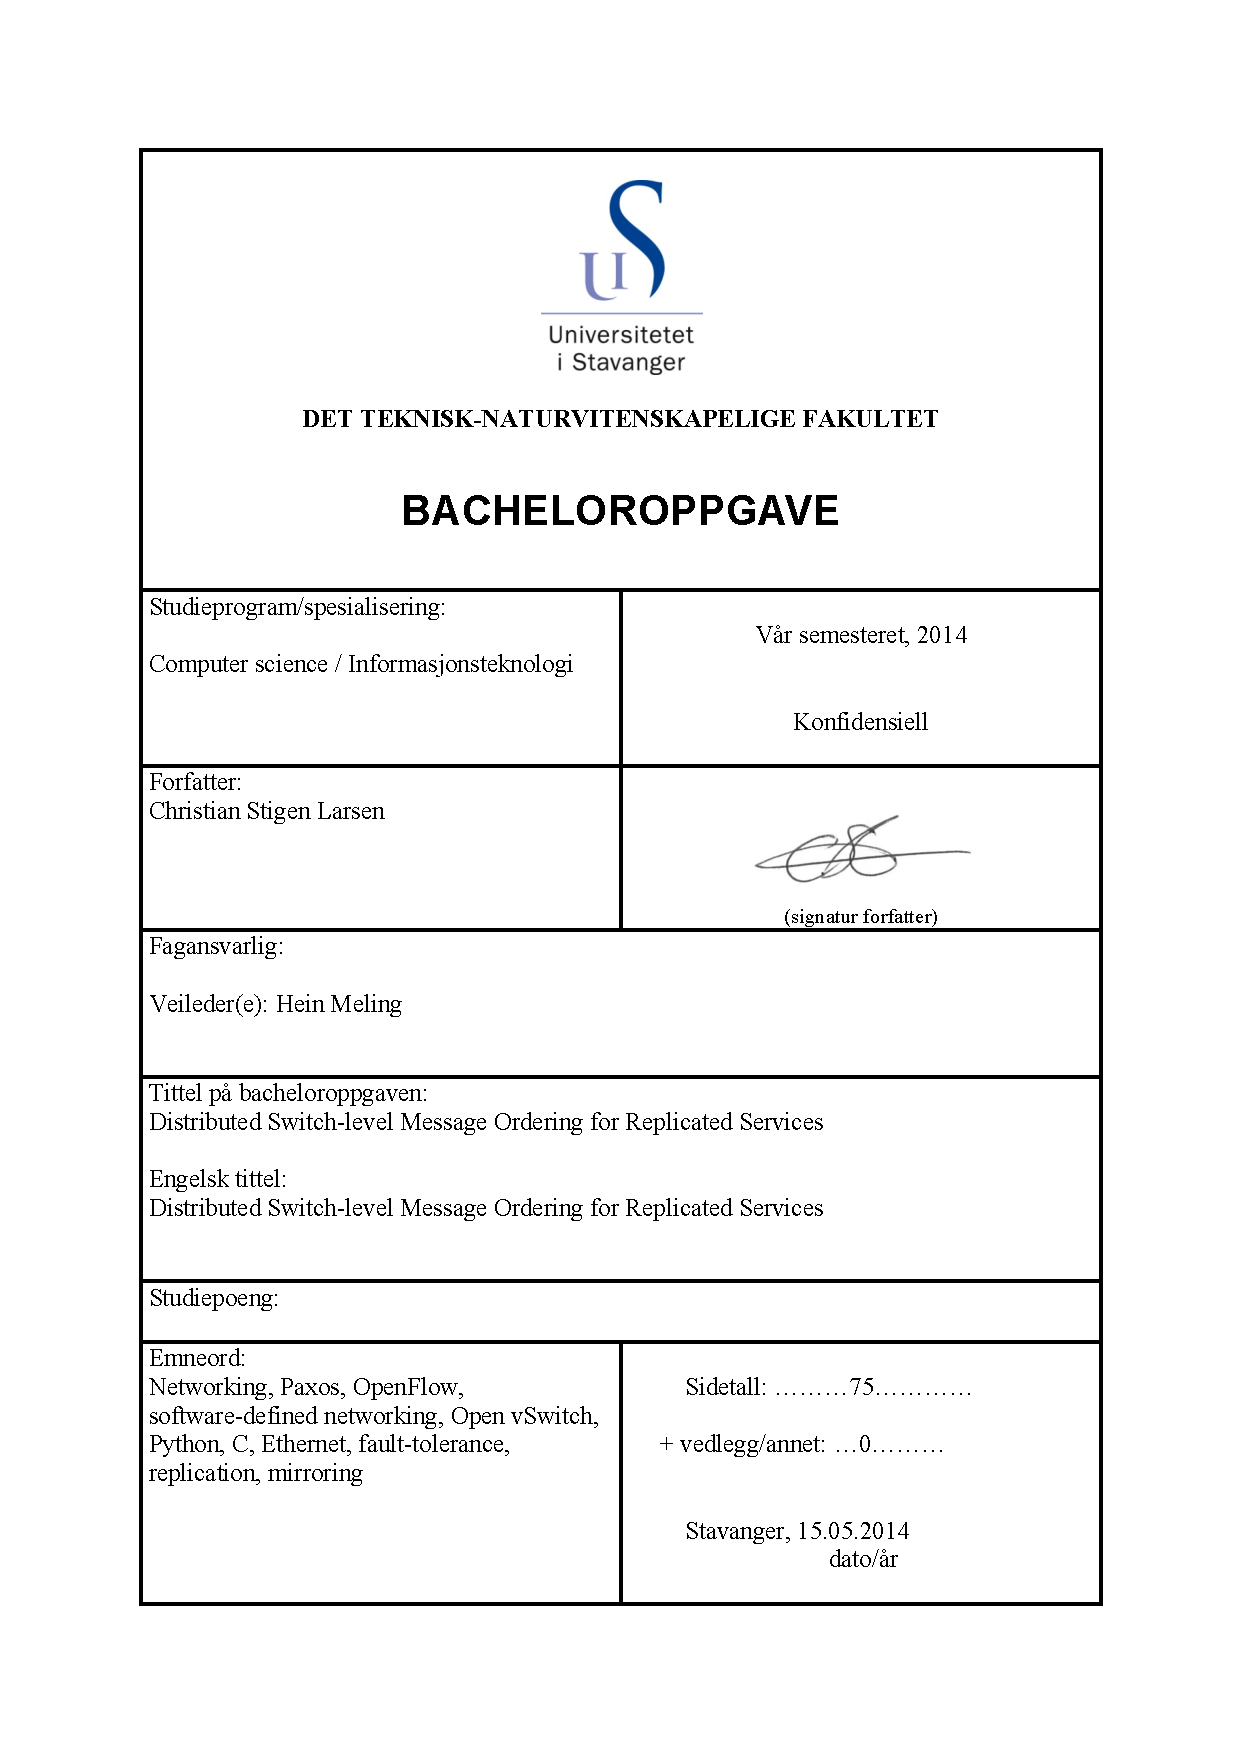
\includepdf[pages={1}]{forside.pdf}
  \maketitle
  \begin{abstract}

\todo{Dette er bare et førsteutkast! Må forbedres.}

Sofware-defined networking (SDN) decouples the control plane from the
forwarding plane in switches, making it possible to create controllers in
software.
%
This has made it easier to build arbitrarily advanced networks, such as
networks that self-optimize for low power-consumption
\cite{Heller:2010:ESE:1855711.1855728}, cloud networks that route live
traffic to moving virtual machines \cite{erickson2008demonstration} as well
as making it possible to test out new networking protocols using simulators
on a laptop.

A trend in the computing industry is that more services are moved to the
Cloud, reaching a larger number of users.
%
Thus, it becomes more important that these services remain available despite
failure of individual machines, calling for distributed service replication.
%
A huge body of research in the distributed computing community have been
devoted to coming up with protocols that guarantee strong consistency among
the replicas of such a service.
%
The most cited paper on network resilience is the Paxos algorithm
\cite{Lam01} for message ordering.

By extending the OpenFlow protocol, we have implemented steady-phase Paxos
on a software switch, making it possible for controllers to compose
flows that leverage the message ordering guarantees of Paxos as a
constituent element.
%
As a demonstration of its use, we have built a system where UDP-based
services are replicated using Paxos transparently.

We conclude that the system shows promise and may be more efficient than
Paxos middleware software for certain network topologies.
%
While the system handles replication of UDP services, TCP may be harder to
support.

\todo{Konklusjon er ikke ferdig}


\end{abstract}

  \cleardoublepage% especially in a document where chapters start at right-hand pages
\phantomsection% for an anchor if you use hyperref
\chapter*{Acknowledgments}% for the actuall unnumbered heading
\thispagestyle{empty}% or plain etc.
\markboth{Acknowledgments}{Acknowledgments}% relevant depending on page sty

I would like to thank my thesis advisor Hein Meling for his close
collaboration, guidance, patience and insightful comments throughout this
work.
%
Hein approached me with the fascinating idea of putting Paxos in the
switch, and I thank him not only for letting me explore this problem, but
also for getting me hooked on software-defined networking.

Multi-Paxos would not have made it into the implementation without the
clear tutorial given by doctoral student Tormod Erevik Lea.

During my modifications of Open vSwitch, I received helpful advice from
its friendly community on the project mailing list.

Finally, none of this would be possible without my amazing fiancée Siri.

While I spent my days at work and University, she had the overwhelming
pleasure of taking care of our two lovely children, Mari and Bjørn.

Thank you for helping me achieve a long-sought dream: I dedicate this
thesis to you.


  \listoftodos % TODO: Remove when finished
  \listoftables
  \listoffigures
  \listofalgorithms\addcontentsline{toc}{chapter}{List of Algorithms}
  \lstlistoflistings\addcontentsline{toc}{chapter}{Listings}

  \tableofcontents

  % Should be after ToC, according to University rules
  %%% Only the acronyms actually referenced in the text will be shown here.

\chapter{Acronyms}
\begin{acronym}
\acro{SDN}{Software defined networking}
\acro{TCP} {Transmission control protocol}
\end{acronym}


  \chapter{Introduction}

Around 2008, \textbf{\acf{SDN}}\index{software-defined networking}
\cite{Casado:2005:VNS:1047344.1047383} emerged from research at
Berkeley\index{Berkeley} and
Stanford\index{Stanford} as a way to enable networks to be defined and managed using
software. One model of \acs{SDN} is \textit{OpenFlow}\todo{Cite!}, which
decouples the control plane\index{control plane} from the forwarding
plane\index{forwarding plane}\index{data plane|see{forwarding plane}} in a
switch, moving it out of the physical switch to an external controller node.
It enables one to implement the controller in software.

Although invented quite recently, software-defined networking is already
being heavily used both in academia and industry.  Google\index{Google}, for instance, are
using OpenFlow to ease deployment and increase utilization in their backbone
networks\index{backbone network} \cite{crabbe2012sdn} and Stanford has deployed several
OpenFlow-controlled networks on their university network.

In March 2013, IDC\index{IDC} \todo{finn ut hva det står for} projected that the SDN market would
  reach \${}3.7 billion by 2016, capturing a 35\%{} share of the switching
  market \cite{Kirkpatrick:2013:SN:2500468.2500473}.
\todo{Skriv om denne setningen, den er tatt nesten direkte fra artikkelen!}

OpenFlow is detailed in \vref{chapter:background.openflow}.

\textbf{Paxos}\index{Paxos} \cite{Lamport:1998:PP:279227.279229} is a
family of distributed, fault-tolerant consensus algorithms.  It allows
network nodes to reach \textit{agreement} even in the face of intermittent
network failures.  For example, one can design a database system using Paxos
to make sure that transactions are executed in the same order on all nodes.

Originally published by Leslie Lamport\index{Lamport, Leslie} in 1989, Paxos
has spawned numerous extensions, including cheap Paxos,
\index{cheap Paxos}\index{Paxos!cheap Paxos} fast Paxos
\index{fast Paxos}\index{Paxos!fast Paxos} and Byzantine
\index{Paxos!Byzantine Paxos}\index{Byzantine Paxos}, fault-tolerant variants.

It is discussed in \vref{chapter:background.paxos}.

\textbf{Our aim} is to build an efficient, \textit{Paxos-enabled software defined
network}.  Paxos will be implemented on OpenFlow switches to guarantee that
packets sent to all of their connected nodes are sent in the same order.
These end-hosts can run any networking service and leverage the benefits of
Paxos without needing to handle any details of the algorithm.

\section{Hypothesis}

For simplicity, we will constrain our scope to a few primitives of
classic crash Paxos\index{Paxos!classic crash} in \textit{phase two},
where we have steady-state
flow\index{Paxos!steady-state flow} with no failures\index{Paxos!failure}.

Furthermore, we want to look at opportunities for increasing networking
performance by moving parts of the Paxos from the control
plane\index{control plane} down to the switches' forwarding
plane\index{forwarding plane}.

We will implement this in progressive stages:

\begin{enumerate}
  \item Implement Paxos entirely in controllers connected to an OpenFlow
  switch.

  \item Extend OpenFlow and Open vSwitch so we can execute Paxos in the
  forwarding plane of the switch.

  \item Move parts of the Paxos implementation down to the forwarding plane
  (OpenFlow \textit{flow tables}), achieving a good balance of performance and
  programming maintainability
\end{enumerate}

Our hypothesis is two-fold:

\begin{enumerate}
\item Network nodes can leverage Paxos guarantees \textit{transparently} by
implementing it on the software switches using OpenFlow.
\item We can achieve good relative performance by moving parts of the
implementation from the OpenFlow controllers down to the software switches.
\end{enumerate}

We aim to build a proof-of-concept system backing up these claims.  The
thesis will therefore be a study of \textit{feasibility}.

\section{Overview}

\todo{Flytt dette inn i teksten over, trenger ikke være egen section.}
We discuss the theoretical background needed to understand this thesis in
chapter \ref{chapter:background} \vpageref{chapter:background}.  If you already know \acs{SDN},
OpenFlow and Paxos, you can skip this chapter.

Then we look at what OpenFlow can offer us in chapter
\ref{chapter:details.openflow}
\vpageref{chapter:details.openflow}, detail what Paxos requires for
implementation in chapter \ref{chapter:details.simplified.paxos} 
\vpageref{chapter:details.simplified.paxos} and propose a
design based on this in chapter \ref{chapter:design} \vpageref{chapter:design}.
\todo{Sjekk at linker stemmer, kan gjerne forenkles også + forbedres}

Finally, we .... blabla ... look at benchmarks and conclude in chapter
\ref{chapter:conclusion} \vpageref{chapter:conclusion}.

\section{Scope}

\todo{Skriv mere og bedre}

We will only look at a simplified version of Paxos in which we only
implement accept and learn messages. We ignore liveness checking such as
heartbeats. We ignore implementing the expanded OpenFlow features in the
network protocol and controller. We only look at steady state Paxos.
We assume switches are co-located. etc etc etc.

We also ignore the fact that if a switch goes down and back up again, it
will need to rejoin the Paxos network and its end-hosts need to synchronize
state\index{synchronization} (or just copy the state from a host on another switch).

\section{Topology}

\todo{Kan kanskje flyttes opp til hypothesis? Vis først HVA vi vil gjøre, og
  så hypotese}

Here we present what we want to achieve.  First, let's look at the situation
for one switch\index{Paxos!topology}.

\begin{figure}[H]
  \centering
  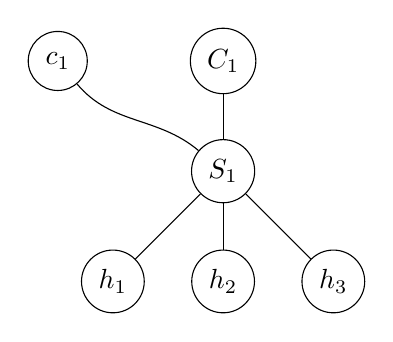
\begin{tikzpicture}[
      every node/.style={draw, circle, minimum width=0.75cm},
      x=0.7cm,
      y=0.7cm]
    \node (c1)    at (-3,  2) {$c_1$};
    \node (ctrl1) at ( 0,  2) {$C_1$};
    \node (S1)    at ( 0,  0) {$S_1$};
    \node (h1)    at (-2, -2) {$h_1$};
    \node (h2)    at ( 0, -2) {$h_2$};
    \node (h3)    at ( 2, -2) {$h_3$};

    \draw (c1) to[out=310,in=140] (S1);
    \draw (S1) -- (ctrl1);
    \draw (S1) -- (h1);
    \draw (S1) -- (h2);
    \draw (S1) -- (h3);

  \end{tikzpicture}
  \caption{A single switch $S_1$ with its controller $C_1$, end-hosts
    $h_1, h_2, h_3$ and one WAN-side client $c_1$.}
  \label{figure:graph.single.switch}
\end{figure}

For an explanation of our nomenclature\index{nomenclature}, we will always
talk about \textit{clients} as being remote hosts on the \ac{WAN} side.

The clients\index{client} are supposed to be placed on the \ac{WAN}---but they are actually
just ordinary hosts on each switch.  We just \textit{pretend} they are
placed on the \acs{WAN}\index{wide-area network}.  It really doesn't matter, though, as all of their
communication goes through each respective switch.

The \textit{end-hosts}\index{end-host} are nodes connected to a single
switch and running services such as key-value stores\index{key-value store},
lock-servers\index{lock-server}, logging servers\index{log server},
databases\index{database}, and so on.

Here is the situation with three switches---the minimum number nodes we need
in a Paxos system.  We have added all-to-all links between the switches in
case any one of them should go down.

\begin{figure}[H]
  \centering
  \begin{tikzpicture}[every node/.style={draw, circle},x=0.7cm,y=0.7cm]
    \foreach \n in {1,2,3} {
      \pgfmathsetmacro\x{(\n-2)*6}
      \node (c\n)    at (\x - 2,  2) {$c_\n$};
      \node (ctrl\n) at (\x ,  2) {$C_\n$};
      \node (S\n)    at (\x ,  0) {$S_\n$};

      \draw (c\n) to[out=305,in=125] (S\n);
      \draw (S\n) -- (ctrl\n);

      \foreach \h in {1,2,3} {
        \pgfmathsetmacro\pos{(\h - 2)*2}
        \pgfmathtruncatemacro\num{((\n - 1)*3) + int(\h)}
        \node (h\num) at (\x + \pos, -2) {$h_{\num}$};
        \draw (S\n) -- (h\num);
      }

    }

    % Links between switches
    \draw (S1) to[out=-10,in=190] (S2);
    \draw (S2) to[out=-10,in=190] (S3);
    \draw [dashed] (S1) to[out=-15,in=195] (S3);

  \end{tikzpicture}
  \caption{Three switches $S_1, S_2, S_3$ with controllers $C_1, C_2, C_3$ acting as Paxos nodes.
           The dashed line between $S_1$ and $S_3$ is a possible \textit{fail-over link}.}
  \label{figure:graph.three.switches}
\end{figure}
\todo{Merk at vi kommer til å ha én public IP-adresse for klienter! Så
      må kanskje vise det på en måte (eller bare nevne det)}

The point is that these services will be mirrored by the use of our
Paxos-enabled switches.  For our purposes, we will assume that the services
on these hosts are \textit{deterministic}\index{deterministic}\footnote{Or,
more correctly, \textit{referentially transparent}\index{referential
transparency}.} in the sense that the parameters uniquely determine the
state of the service after being processed---if two hosts running the
same service receive the exact same packet, their state will be
identical after having processed it.  This is a prerequisite for our
system.  The OpenFlow switches, running Paxos, will only make sure that
packets are delivered in the \textit{same order} to the end-hosts.

\section{Viability}

Why would such a system be useful? Consider the situation of implementing
Paxos in code on some servers, running services such as key-value
stores\index{key-value store}, etc.

\begin{figure}[H]
  \centering
  \begin{tikzpicture}[every node/.style={draw, circle},x=0.7cm,y=0.7cm]

    % For each switch ...
    \foreach \n in {1,2,3} {
      \pgfmathsetmacro\x{(\n-2)*6}
      \node (ctrl\n) at (\x ,  2) {$C_\n$};
      \node (S\n)    at (\x ,  0) {$S_\n$};

      \draw (S\n) -- (ctrl\n);

      % For each host ...
      \foreach \h in {1,2,3} {
        \pgfmathsetmacro\pos{(\h - 2)*2}
        \pgfmathtruncatemacro\num{((\n - 1)*3) + int(\h)}

        % Host node
        \node (h\num) at (\x + \pos, -2) {$h_{\num}$};
        \draw (S\n) -- (h\num);

        % Paxos node
        \node [very thick] (P\num) at (\x + \pos, -3.75) {$P$};
        \draw [dashed] (h\num) -- (P\num);
      }
    }

    % Links between switches
    \draw (S1) to[out=-10,in=190] (S2);
    \draw (S2) to[out=-10,in=190] (S3);
    \draw [dashed] (S1) to[out=-15,in=195] (S3);

  \end{tikzpicture}
  \caption{Support for Paxos on the servers $h_1, \dots, h_3$ requires a
    copy of the Paxos code $P$ on each server.}
  \label{figure:paxos.on.servers}
\end{figure}

Here, each server needs to have an implementation of Paxos in code (shown as
$P$ in figure \ref{figure:paxos.on.servers}).  It means the software
developer has to specifically add support for Paxos when designing the
server code, tailoring it for the particular service.  All Paxos handling
must be done at a high networking layer\index{networking layers}---most
likely in the application layer\index{application layer} at the very top.

Now consider the situation where the switch provides Paxos
capabilities\index{Paxos!on switch} (figure \ref{figure:paxos.on.switches}).

\begin{figure}[H]
  \centering
  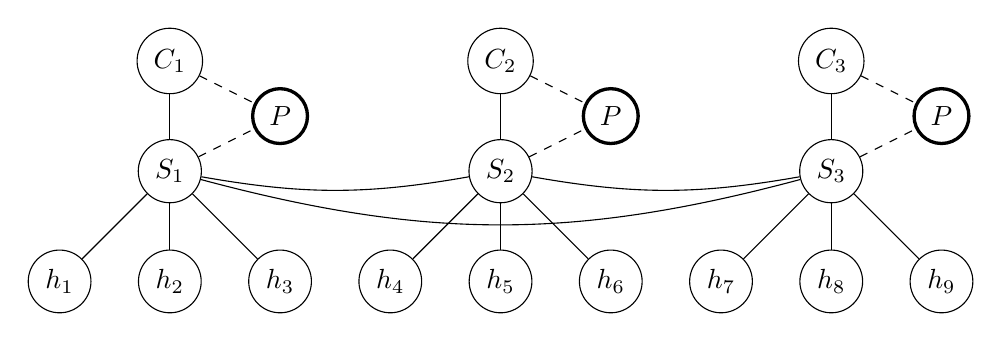
\begin{tikzpicture}[every node/.style={draw, circle},x=0.7cm,y=0.7cm]

    % For each switch ...
    \foreach \n in {1,2,3} {
      \pgfmathsetmacro\x{(\n-2)*6}
      \node (ctrl\n) at (\x ,  2) {$C_\n$};
      \node (S\n)    at (\x ,  0) {$S_\n$};

      \draw (S\n) -- (ctrl\n);

      % Paxos node
      \node [very thick] (P\n) at (\x + 2, 1) {$P$};
      \draw [dashed] (S\n) -- (P\n);
      \draw [dashed] (ctrl\n) -- (P\n);

      % For each host ...
      \foreach \h in {1,2,3} {
        \pgfmathsetmacro\pos{(\h - 2)*2}
        \pgfmathtruncatemacro\num{((\n - 1)*3) + int(\h)}

        % Host node
        \node (h\num) at (\x + \pos, -2) {$h_{\num}$};
        \draw (S\n) -- (h\num);
      }
    }

    % Links between switches
    \draw (S1) to[out=-10,in=190] (S2);
    \draw (S2) to[out=-10,in=190] (S3);
    \draw (S1) to[out=-15,in=195] (S3);

  \end{tikzpicture}
  \caption{Paxos ($P$) on the switches $S_1, S_2, S_3$ mitigates the need for special code on the servers.}
  \label{figure:paxos.on.switches}
\end{figure}

In figure \ref{figure:paxos.on.switches}, the switches themselves (and their
controllers\index{Paxos!controller}) enable
support for Paxos.\footnote{We have moved the servers to several switches
to indicate a distributed nature between the switches.
Paxos on a single switch would not be very useful, as that would be a single
point of failure and---after all---be the sole decision point for message
ordering.}
This should let the servers be oblivious of the fact that Paxos is used to
enable ordering of packet arrival to them.

Besides, Paxos is now run at a much lower networking level\index{networking
layers} and at the point where switching is done---there will be less hops
for each packet.

Of course, there are pros and cons for each scenario.
When implementing Paxos, one can often take advantage of
the particular way each server operates. Sometimes one actually
\textit{needs} to know this to implement Paxos.  Therefore, an
implementation of Paxos in each server's code base would be beneficial.

Also, it means that we need to run code on the switches themselves. This
gives rise to a wide range of non-functional requirements for the code.
For instance, code that runs for too long must be
preempted\index{preemption} to let the switch smoothly handle other
requests. Not doing so may result in packet loss, high latency or
worse---complete incapacity to serve data. Besides, switches do not normally
have hardware capable of running \textit{generic} software fast. They
usually have highly optimized hardware to do some of the heavy-lifting.

On the other hand, in our scenario, we can potentially add support for
message ordering through Paxos on servers that does not already support it.
The kinds of services that this would work on is for systems that are
deterministic in nature: The same input (or client packet) on any server
would produce the same internal state and output.
%
But there is a big class of software that has this behaviour:  Key-value
stores, logging servers, relational databases and so on.\footnote{But not
lock servers, because a lock can only be held by one server at a time.}

The only thing our model does not cover is the situation where a switch goes
completely down.
In that case, each connected server should start
synchronizing their internal state with any of the others that have been up.
\todo{Mangler jo også leader election og failures. Må få
  fram at jeg mener at KONSEPTET støtter mange ting, men ikke vår
    IMPLEMENTASJON.}

All in all, we believe this is a viable experiment with practical benefits.
Indeed, using a software-based approach for switches lets us test our model
on \textit{any} existing piece of server software.

Moreover, we also intend to show how one can optimize the performance of
this model further, by moving parts of the Paxos implementation down into
the switches' flow tables.  This should have a big impact, because Paxos
handling is done at a lower networking layer and closer to the central network
components than what would be the case with Paxos in the server's code.

\todo{Føler vi trenger flere, sterkere argumenter.}

  \chapter{Background}
\label{chapter:background}

In chapter \ref{chapter:introduction} we stated our thesis goal of offering
Paxos at the networking-level and building a distributed replication system
on top of it.
%
Here, we will present the background material for algorithms and technology
we will use in the rest of this thesis.

\section{OpenFlow}
\label{chapter:openflow.background}

As mentioned in chapter \ref{chapter:introduction}, the core idea of
\acs{SDN} is to dissociate the controller from the switch, enabling software
developers to ``program the network''.  This is illustrated in figures
\ref{figure:coupling.planes} and \vref{figure:decoupling.planes}.

OpenFlow \cite{McKeown:2008:OEI:1355734.1355746,openflow-1.0} is one of
several ways to enable \acf{SDN}
%
It is a specification of a messaging protocol for the interaction between
a switch and controller, detailing what kind of actions that can be
performed by each of these components.
%
Examples of \ac{SDN} solutions predating OpenFlow are SANE
\cite{Casado:2006:SPA:1267336.1267346}, Ethane
\cite{Casado:2007:ETC:1282427.1282382}, 4D
\cite{Greenberg:2005:CSA:1096536.1096541}.

In OpenFlow, the controller is a piece of software can inspect packets and
send commands down to the switch.  It can instruct the switch perform actions like
forwarding a packet to an output port going to another switch, changing
header fields, drop it and so on.
%
Additionally, the switch can be set up to perform such actions by itself,
using a \textit{flow table}.  This is what we have previously referred to as
the \textit{forwarding plane}, and as highly performant in comparison to
handling each individual packet in the controller.

OpenFlow controllers can be written in any programming language that offers
an OpenFlow framework.  While the OpenFlow switches are usually also
implemented in software, several vendors now ship hardware switches that
support the OpenFlow protocol.

\subsection{The Flow Table}
\label{chapter:theory.flow.table}

The aforementioned flow table consists of several flow
entries---colloquially called \textit{flows}.
%
These contain rules for matching packets and actions to perform when there
is a match.
%
In addition there are several counters used for collecting various
statistical metrics (e.g., how many times a flow has been executed) and
timeouts that dictate how long an entry will exist in the table.

\begin{figure}
  \centering
  \begin{subfigure}[t]{0.45\textwidth}
    \centering
    \begin{tikzpicture}[every node/.style={draw, circle},
                        node distance=2.5cm]
      \node [rectangle,
             rounded corners,
             minimum width=3cm,
             minimum height=1cm] (Sbig) at (0,0) {};

      \node [draw=none] (S) at (0,0) {$S$};
      \node [right=0.25cm of S] (C) {$C$};
      \node [left=0.25cm of S] (F) {$F$};

      % Add invisible node from figure B so that they align vertically
      \node [draw=none] (vspacer) [above of=S] {};

      \node (h1) [dashed, below left of=S] {};
      \node (h2) [dashed, below of=S] {};
      \node (h3) [dashed, below right of=S] {};

      \draw [dashed] (Sbig) -- (h1);
      \draw [dashed] (Sbig) -- (h2);
      \draw [dashed] (Sbig) -- (h3);

    \end{tikzpicture}
    \caption{A typical switch $S$ combines the control and
      forwarding planes ($C$ and $F$) on the same device.
        The control plane
        $C$ is usually locked down by the vendor and inaccessible to users.}
    \label{figure:coupling.planes}
  \end{subfigure}%
  \hspace*{0.1\textwidth}%
  \begin{subfigure}[t]{0.45\textwidth}
    \centering
    \begin{tikzpicture}[every node/.style={draw, circle},
                        node distance=2.5cm]

      \node [rectangle,
             rounded corners,
             minimum width=3cm,
             minimum height=1cm] (S) {$S$};

      \node (T) [above of=S] {$C$};
      \node (h1) [dashed, below left of=S] {};
      \node (h2) [dashed, below of=S] {};
      \node (h3) [dashed, below right of=S] {};

      \node (FlowTable) [left=-0.9cm of S] {$F$};

      \draw (T) -- (S);
      \draw [dashed] (S) -- (h1);
      \draw [dashed] (S) -- (h2);
      \draw [dashed] (S) -- (h3);

    \end{tikzpicture}
    \caption{\ac{SDN} decouples the control plane $C$ from the forwarding
      plane $F$ by moving it out of the switch $S$ to an external network
        node.  The \textit{OpenFlow protocol} enables communication between
        $S$ and $C$, making it possible to implement $C$ in software on an
        ordinary computer. In OpenFlow, the connection between $S$ and $C$ is encrypted.}
    \label{figure:decoupling.planes}
  \end{subfigure}
\end{figure}

When a switch receives a packet, it will try to match it with entries in
the flow table (table \vref{openflow.flow.entry.spec}).
%
Each flow contains a \textit{matching pattern}\index{OpenFlow!matching} and
a set of actions\index{OpenFlow!actions}\index{flow table} to perform in
case there is a match.
%
The actions can be to rewrite a header field, forward the
packet to a port, drop it and so on.
%
If a packet does not match any flows, the switch will forward a buffer ID
and packet headers to the controller $C_1$ on a secure channel.

\begin{table}[H]
  \centering
  \begin{tabular}{|c|c|c|}
    \hline \textbf{Header fields} &
           \textbf{Counters} &
           \textbf{Actions} \\
    \hline \dots & \dots & \dots \\
  \end{tabular}

  \caption{The OpenFlow 1.0 flow table.}
  \label{openflow.flow.entry.spec}
\end{table}

The controller can then decide what to do with the packet.  Using the
OpenFlow protocol, it can issue immediate actions to the switch or install
flows, so the switch can operate on its own.

The flow tables are initially empty, meaning that all packets are by default
sent to the controller.  During this phase, the controller will
explicitly handle every packet.  At the same time, it will incrementally
build up an internal map of the network.  As the map forms, it can start
installing flows in the switch.

For instance, if a controller learns the port numbers for a pair of
addresses, it can instruct the switch to automatically forward packets to
their appropriate output ports when they communicate.
%
If a packet's destination port is unknown, the controller can
\textit{rebroadcast}\index{rebroadcasting} it out on all ports except where
it came from, knowing that only designated receivers will accept the packet.
%
What we have described here is a \textit{learning switch}, and is explained
in detail in chapter \vref{chapter:l2.learning.switch}.

Along with each flow entry is an associated set of timeouts.  Flows are
removed from the flow table when they time out.
%
This serves several purposes.  First of all, it makes sure that flow tables
do not fill up quickly.  Secondly, because flows---and packets---are
transient by nature, controllers will be given the chance to update rules
based on changes in the network.
%
Finally, this mode of operation adheres to the principle of autonomous
operation\index{autonomous operation} commonly seen in networking devices.

Well-designed controllers should not need elaborate configuration to work.
So while they initially do all the heavy-lifting by themselves, they will
offload work to the switches, who can then dispatch packets very quickly.

\subsection{Applications of OpenFlow}

We would like to briefly mention a few real-world uses of OpenFlow.

Researchers at Stanford\index{Stanford}
built an OpenFlow network that was able to migrate a virtual video game
server \ac{VM} from California to Japan---while it was running, without
interruption, using the \textit{same} IP-address
\cite{erickson2008demonstration} \cite{kobayashi2013maturing}.

Google are using OpenFlow in their backbone network to increase utilization
\cite{crabbe2012sdn} and is an official member of the governing institution
of OpenFlow, the \ac{ONF}.

The Open Networking Foundation released the first specification of OpenFlow
in 2009 and continually publish point versions, errata and new versions
\cite{openflow-1.0,openflow-1.0.1,openflow-1.0.2,openflow-1.1,openflow-1.2,openflow-1.3,openflow-1.4}.
The most recent one, at the time of writing, is version
1.4\index{OpenFLow!versions}.

\section{Mininet, POX and Open vSwitch}
\label{chapter:mininet}

Mininet \cite{github:mininet} is an open source network simulator that
supports OpenFlow.
%
Using the Python programming language, one can deploy virtual networks on a
laptop, configuring link speeds, percentage of packet loss and so on.
%
Controllers are written using the POX \cite{github:pox} OpenFlow framework.

At the bottom of all this is the Open vSwitch program \cite{github:ovs}.
It is a powerful software switch used by many cloud providers.
It supports most of the OpenFlow functionality, and runs both as a Linux
kernel module and in user space.
%
Open vSwitch is written by many of contributors of the OpenFlow
specifications, and the three projects share close ties.

Together, they form a powerful combination of software that makes it easy
to experiment with networking technology.  We have used them for our thesis
implementation.

\section{Paxos}
\label{chapter:background.paxos}

Paxos \cite{Lam01, Lamport:1998:PP:279227.279229} is a family of
fault-tolerant, distributed consensus algorithms, allowing nodes to reach
agreement in the face of intermittent failures.
%
Originally published by Leslie Lamport\index{Lamport, Leslie} in 1989, Paxos
has spawned numerous extensions, including cheap Paxos,
\index{cheap Paxos}\index{Paxos!cheap Paxos} fast Paxos
\index{fast Paxos}\index{Paxos!fast Paxos} and Byzantine
\index{Paxos!Byzantine Paxos}\index{Byzantine Paxos}, fault-tolerant variants.

We will not give a full account of the Paxos algorithm here, but will
mention the main parts that are relevant for this thesis.  For reference, we
will hereafter keep to the description given in \cite{Lam01}.

Paxos consist of two main phases: \textit{Phase one} and \textit{phase 2}.
The first phase consists of choosing a leader among all the Paxos nodes.
This phase continues until a leader has been chosen by the majority.
As we will only focus on phase two, we will not discuss this part further.

Phase two, also called \textit{steady-phase}, is where \textit{message
ordering} takes place.   We say that we want to reach \textit{consensus} on
some \textit{value}.  A \textit{value} can be anything we want a majority of
the nodes to agree on.  For our purposes, it means we want to determine
which packet to next process (i.e., we want to determine the
    \textit{order} in which to process packets).  Paxos nodes will send
Paxos messages to each other, and they contain various parameters.  We will
return to these in section \vref{section:paxos.consensus.algorithm}.

The \textit{Paxos leader} from the first phase will receive a message
somehow---in our case, it will be a client packet that we wish to distribute
and process in-order---send out an \textit{accept} message containing a
\textit{value} to be agreed upon---the value can for example be a packet or
a reference to a packet, for example---and sending out an \textit{accept}
message to its \textit{Paxos slaves}.  Only the leader sends out accept
messages.

When a slave received an accept, it will first see if this is a message that
came from its current leader.  If so, and if it has not seen this message
before, it will send a \textit{learn} message to \textit{all} Paxos nodes,
including itself.

Upon receiving a learn-message, a node will first check if it belongs in the
current \textit{round}---meaning that the message belongs in the current
round with the given leader.  In other words, if the round number contained
in the learn message is less than the node's current round, this was a
message from a previous point in time in which there was
\textit{possibly} another leader.  If the learn has not been seen before, it
will record how many unique learns it has seen.
%
Whenever a node has received learns from a majority of other nodes, it will
start to process a queue of messages in the order specified by the message
parameters.

We will refrain ourselves from discussing \textit{why} the algorithm works,
even in the face of failures.  For such details, we refer to \cite{Lam01,Insane.Paxos}.

This concludes our very brief account of Paxos, and we will return to it in
section \ref{section:paxos.consensus.algorithm}.

  \chapter{Design}

Now that we have discussed the main algorithms and our simplification of
them, we must take a look at what OpenFlow can offer us to reach our goals.

\section{Features in OpenFlow versions 1.0--1.4}

To see how we can enable Paxos functionality in OpenFlow, we need to take a
look at what features it can provide us.

Naturally, we could implement the whole Paxos algorithm in the controller
itself.  Doing so should be quite trivial: One could take an existing
implementation and make some slight modifications to it.  There is in fact
some merit to this idea, because we could deploy systems where most of the
Paxos algorithm is implemented on the controllers, leaving some minor Paxos
code to run on the end--systems (for instance, the end--systems would need
to recognize Paxos LEARN--messages and extract the payload).

However, that would be very inefficient compared to running the entire
algorithm---or parts of it---on the switch.

OpenFlow controllers are meant to set up entries in the flow tables as they
see fit.  In an efficient OpenFlow--system, the
controllers will initially get lots of packets and program the flow tables.
Over time, more work can be performed by the use of flow tables, and so the
controllers will only update the flow tables intermittently.

The flow tables themselves will then be able to match given
packets to the specification and perform actions on them.  These flow tables
are {\em designed} to allow very efficient implementations in hardware.  In
other words, this means that the actions that can be performed are very
simple and far from a fully--fledged programmable system.

Because of this, we need to take a look at what operations we can perform in
OpenFlow.  The versions vary quite a bit on this point, and a lot of
software only support given versions.  So let's get an overview of what is
possible in the different OpenFlow versions.




\section{Limitations in OpenFlow}

By looking at what OpeFlow versions 1.1--1.3 offer, one can see that we can't really
make use of any of the added functionality for running Paxos.  What we need
is the ability to run programs on the switch, which is something OpenFlow
does not support at all.  Neither do their action primitives add up to
anything that could be used for remembering state (such as the current round
number) or executing if--then--else statements.

One possibly solution would be to insert a lot of flow table entries that
each waited for a specific round number.  But that would not be an elegant
or practical solution.

They \textit{do}, however, offer us the ability to implement Paxos entirely
on the controller.  We have actually done this, but one of the stated goals
of this thesis was to move parts of the Paxos code down to the switch
itself.  For this we simply need to be able to run full Turing--equivalent
programming languages.

For remembering state, we looked at the metadata that is available in later
versions of OpenFlow.  However, metadata only exists as the packet is
processed in the pipeline of flow tables, and is erased when the packet
actions are applied at the end.  To remember state, we will need to add a
table to hold such data in the switch.

Finally, we have to look at which OpenFlow versions our software components
support.

Mininet seems to support whatever version of OpenFlow that OpenVSwitch uses,
as this is what it uses as a switch.  OpenVSwitch It supports OpenFlow versions
1.0---1.3 almost fully, but support for 1.4 is flaky, and may crash.  So 1.4
is out of the question.

The most obvious component to look at is POX, our controller
framework in Python, which only supports OpenFlow 1.0\footnote{It does seem
to support some \textit{Nicira extensions}, though.  These are extensions
that were originally added to early OpenFlow versions, but much of it
has been implemented in later versions.  There is also a fork of POX (and other
software projects) written by CPqD that adds support for newer OpenFlow
versions, but we haven't looked at it.}.

But the major point for our decision is what OpenFlow can offer us.
There simply is no way of executing general code, and there is no way to
remember state\footnote{We even investigated whether we could use the
counters to count round numbers or store them in IPv6 addresses, using VLAN
for storing data, etc.  All those ideas turned out to be very hairy to
implement, with a real possibility of not working correctly.}

All in all, we have decided to use OpenFlow 1.0 where applicable and extend
it where needed.  Using the flow table, controller and bytecode is a simple
but good, practical decision.

\section{Decisions}

We have seen that OpenFlow does not offer the capabilities we need to
implement Paxos on the switch.  We could implement Paxos on the controller,
but that would be nearly equivalent to having adding Paxos to the software
running on the end--hosts.

Thus, we have decided to use a combination of OpenFlow flow table rules and
programs running in OpenVSwitch as bytecode compiled fragments to handle the
details of the Paxos algorithms.

\todo{Legg til selve designet her, siden tittelen sier det! Vis hvor vi
bruker flow tables (ikke vis detaljer, det kommer senere), vis
nettverksflyt, vis hvor bytecode blir eksekvert, og hva som kjører på
controller.}

\section{Choice of switch programming language}

\todo{Insert a "defense" of why we chose Forth, and why we didn't implement
everything in OpenFlow}

What we want is to provide \textit{simple} primitives that can be
implemented to run custom code \textit{efficiently} on the
hardware---requiring little memory and few cycles per operation---while
still being useful for other networking protocols.
\todo{back up this statement on the last part}

We think this is a good implementation for fastidious hardware implementors,
but \textit{any} programming language---preferably one that can produce
bytecode---would work just as fine.
\todo{Finn ut hvor jeg snakker om Ngaro og flytt tekst over her.}


  \chapter{Implementation}
\label{chapter:implementation}

Based on the design in chapter \ref{chapter:design}, we will now look at
implementation details.

To be able to run Paxos in the switch, we must first extend the OpenFlow
Switch Specification with a new \textit{Paxos action}.
\index{flows!Paxos action}\index{OpenFlow!Paxos action}%
\index{Paxos!OpenFlow action}%
%
This will allow us to freely \textit{compose} flows that run the
Paxos algorithm as one part of their actions.
%
Finally, we must modify Open vSwitch so that we can run the new action.

\section{Extending the OpenFlow Specification}

As discussed earlier in chapter \ref{chapter:openflow.design}, it would be
impractical to attempt to use existing actions in the OpenFlow specification
to implement the Paxos algorithm.
%
The OpenFlow specifications, as of version 1.4 \cite{openflow-1.4}, are
backward-compatible, meaning that a newer OpenFlow version will support all
features in older ones.  We will therefore choose to extend version 1.0
\cite{openflow-1.0}, because it was the first public version and therefore
the most widely supported.

The idea is to add a new \textit{Paxos action} with a parameters 
specifying whether to run the \textit{On Client}, \textit{On Accept} or 
\textit{On Learn} parts of the Paxos algorithm given in chapter
\vref{ch:simplifying.paxos}.
%
As shown in \vref{chapter:openflow.background}, we can then specify
precisely what kind of events we want to trigger Paxos ordering for and
combine that with other actions, such as which port the output should go to.

The part of the specification we need to extend is the 
\textit{Flow Action Structures} \cite[pp.~21--22]{openflow-1.0},
and it will be an \textit{optional} action \cite[pp.~3--6]{openflow-1.0}.
%
Listing \ref{listing:ofp10.action.type} shows the modification made to
the C\index{C} enumeration type \texttt{ofp10\_{}action\_{}type} from the
Open vSwitch source
code.\footnote{\texttt{ovs/include/openflow/openflow-1.0.h}}
We have included listing listing:ofp10.action.type as-is because this is how
it is defined in the published OpenFlow specification \cite{openflow-1.0}.
%
The listing is identical to the official specification, except for the
number suffix in \texttt{OFPAT10}.

\begin{lstlisting}[
  caption={Adding the \texttt{OFPAT10\_{}PAXOS} action to the OpenFlow
           specification},
  label={listing:ofp10.action.type}]
enum ofp10_action_type {
    OFPAT10_OUTPUT,             /* Output to switch port. */
    OFPAT10_SET_VLAN_VID,       /* Set the 802.1q VLAN id. */
    OFPAT10_SET_VLAN_PCP,       /* Set the 802.1q priority. */
    OFPAT10_STRIP_VLAN,         /* Strip the 802.1q header. */
    OFPAT10_SET_DL_SRC,         /* Ethernet source address. */
    OFPAT10_SET_DL_DST,         /* Ethernet destination address. */
    OFPAT10_SET_NW_SRC,         /* IP source address. */
    OFPAT10_SET_NW_DST,         /* IP destination address. */
    OFPAT10_SET_NW_TOS,         /* IP ToS (DSCP field, 6 bits). */
    OFPAT10_SET_TP_SRC,         /* TCP/UDP source port. */
    OFPAT10_SET_TP_DST,         /* TCP/UDP destination port. */
    OFPAT10_ENQUEUE,            /* Output to queue. */
    OFPAT10_PAXOS,              /* Extension: Run Paxos algorithm. */
    OFPAT10_VENDOR = 0xffff
};
\end{lstlisting}

The Paxos action has only one parameter: Which part of algorithm
\ref{ch:simplifying.paxos} to run.  The structure of this parameter is given
in listing \ref{listing:ofp10.action.paxos} and its its possible values are
defined in table \ref{table:paxos.event.codes}.
%
All action structures are required to start with the \texttt{type} and
\texttt{len} fields.

\begin{lstlisting}[
  caption={The \texttt{OFPAT10\_{}PAXOS} parameters},
  label={listing:ofp10.action.paxos}]
struct ofp10_action_paxos {
    ovs_be16 type;            /* Required: OFPAT10_PAXOS. */
    ovs_be16 len;             /* Required: Length is 8. */
    ovs_be32 paxos_event;
};
OFP_ASSERT(sizeof(struct ofp10_action_paxos) == 8);
\end{lstlisting}

As we can see, \texttt{paxos\_{}event} is encoded as a big-endian, unsigned
32-bit integer.
%
Its possible values are given in table \ref{table:paxos.event.codes}.

\begin{table}[H]
  \centering
  \begin{tabular}{|c|l|c|l|}
    \hline
      \textbf{Value} &
      \textbf{Meaning} &
      \textbf{Algorithm} &
      \textbf{\texttt{ovs-ofctl} argument}
      \\

    \hline
      \texttt{0x7A01} &
      Run ``On Accept'' &
      \ref{algorithm:paxos.simple.acceptor} &
      \texttt{paxos:onaccept}
      \\

    \hline
      \texttt{0x7A02} &
      Run ``On Learn'' &
      \ref{algorithm:paxos.simple.learner} &
      \texttt{paxos:onlearn}
      \\

    \hline
      \texttt{0x7A40} &
      Run ``On Client'' &
      \ref{algorithm:paxos.simple.client} &
      \texttt{paxos:onclient}
      \\

    \hline
  \end{tabular}
  \caption{Possible values for \texttt{paxos\_{}event} in listing
           \ref{listing:ofp10.action.paxos}}
  \label{table:paxos.event.codes}
\end{table}

The values in table \ref{table:paxos.event.codes} have been chosen
to correspond to the Ethernet types given
in table \vref{table:paxos.ethernet.type.encoding}, although they
could have been simply zero, one and two.
%
The last column contains the command-line arguments that will be
accepted by \texttt{ovs-ofctl} when adding flows.

Because of the thesis scope, we have only added a single action parameter
\texttt{paxos\_type}.
%
In a production environment, however, one would likely need several more.
%
For example, it could be useful to distinguish between different
\textit{sets} of Paxos nodes so they could operate independently of each
other on the same network.
%
Here, we have only \textit{one} set of Paxos nodes who all have the same
leader.

\subsection{Modifications to Open vSwitch}

As mentioned in section \vref{chapter:mininet}, the component in our system
that actually executes OpenFlow actions is \textit{Open vSwitch}.
To fully implement the new Paxos OpenFlow action, we need to do this in Open
vSwitch.  Details can be found in section \vref{chapter:compiling.ovs}.

Looking at table table \vref{table:paxos.event.codes}, the rightmost column
(\textbf{\texttt{ovs-ofctl} argument}) contains arguments to the Open
vSwitch command-line tool \texttt{ovs-ofctl}, that can be used to program
Paxos actions as smaller parts of bigger flows.

To demonstrate how elegantly one can set up flows that use Paxos ordering,
consider the below example for installing a flow on the switch
\texttt{S1}.

\begin{Verbatim}
sudo ovs-ofctl add-flow S1 \
               in_port=3,dl_type=0x7a40,actions=paxos:onclient,output:5
\end{Verbatim}

The above command installs a new flow entry on \texttt{S1}, matching packets
coming in on port 3 with the Ethernet type \texttt{0x7a40}.  
Referring to table \vref{table:paxos.event.codes}, we see that this flow
will match on packets of type \texttt{CLIENT}.

Furthermore, under \texttt{actions=}, we instruct Open vSwitch to run the
Paxos action with the parameter \texttt{onclient}.  This means that for
matching packets, Open vSwitch will dispatch the packet to the \textit{on
client} function (the argument \texttt{paxos:onclient}), described in
chapter \vref{chapter:paxos.client.message} and algorithm
\vref{algorithm:paxos.simple.client}.
%
This algorithm will output an accept message to output port 5
(\texttt{output:5})
If we want to explicitly set the destination address of the packet, one can
just prepend the output with the modification action
\texttt{mod\_dl\_dst=a1:b2:c3:d4:e5:f6}.
To send out on several ports, one just needs to add more \texttt{output:<N>}
actions, or the packet can be flooded on all ports with
\texttt{output:flood}.

What we are doing here is programming the switch's flow table using Paxos
primitives as constituent elements.  For the actual implementation, we refer
to the appendix, section \vref{chapter:compiling.ovs}.

We have implemented all of the actions in table
\ref{table:paxos.event.codes}, including multi-Paxos storage of packets in
slots, but with the important exception of the queue processing (algorithm
\ref{algorithm:paxos.simple.learner}, section
\ref{ch:simplifying.paxos}).

The above command translates client packets to Paxos \texttt{ACCEPT}
packets.  For a Paxos node on another switch, we can simply use the
\texttt{paxos:onaccept} action.  Since switch $S_2$ of figure
\vref{figure:paxos.on.switches} may receive Paxos messages from both $S_1$
and $S_3$, we may want to only react on packets that are explicitly
addressed to $S_2$.
%
To do so, assuming the MAC-address is \texttt{22:22:22:22:22:22}, one may
simply add a matching pattern for it, along with the obligatory check for
the Ethernet type field corresponding to an accept message
(\texttt{0x7A01}):

\begin{Verbatim}
sudo ovs-ofctl add-flow S2 \
    dl_src=11:11:11:11:11:11,\         # match from leader S1
    dl_dst=22:22:22:22:22:22,\         # match S2 MAC-address
    dl_type=0x7a01,\                   # match ACCEPT message
    actions=paxos:onaccept,\           # run "On Accept"
    mod_dl_src=22:22:22:22:22:22,\     # set source MAC address
    mod_dl_dst=33:33:33:33:33:33,\     # set destination MAC to S3
    output:5,\                         # output to port 5
    mod_dl_dst=11:11:11:11:11:11,\     # set destination MAC to S1
    output:1                           # output to port 1
\end{Verbatim}

The flow above is an \textit{actual} flow that we used---and verified to
work---in our network simulator.  If all conditions of algorithm
\ref{algorithm:paxos.simple.acceptor} are met, this flow wil send out a
learn message to $S_1$ and $S_3$.

Comparing this with writing equivalent flows as procedures in Python, this
is \textit{vastly} easier to do.  An \textit{excerpt} from the code for
accept-hanling in the Python controller is given below.

\begin{lstlisting}[
  caption={Shortened excerpt of Python code for handling Paxos accept messages},
  label={listing:python.accept}]
def on_accept(self, event, message):
  n, seqno, v = PaxosMessage.unpack_accept(message)
  src, dst = self.get_ether_addrs(event)

  # From leader?
  if src != self.leader.mac:
    return EventHalt # drop message

  slot = self.state.slots.get_slot(seqno)

  if n >= self.state.crnd and n != slot.vrnd:
    slot.vrnd = n
    slot.vval = v

    # Send learns to all
    for mac in self.state.ordered_nodes(self.mac):
      self.send_learn(mac, n, seqno, self.lookup_port(mac))

  return EventHalt
\end{lstlisting}

The code in the listing above is a shortened version of the
actual implementation.
%
Of course, we have had to actually \textit{implement} the above code in
equivalent C code in Open vSwitch, but the big gain is that the flows are
happening on the switch, and requires no upcall to the controller.


\todo{Flytt resten av kapittelet}

As discussed in \vref{chapter:theory.flow.table}, well-designed controllers
should install flows incrementally as they learn the network topology.
%
We must therefore first implement a system that works entirely without flow
entries. (Dette er en del av design-diskusjon, vi skal bare implementere det
her).

Next, we will implement flows in the system. As discussed previously, this
requires an extension to the OpenFlow-protocol and the switch software we
use, Open vSwitch. \todo{Dette må ha vært diskutert før}

Mer tekst: At vi har, i designet, extenda OpenFlow + Open vSwitch slik at vi
kan kjøre kode. Vi viser implementasjonen her, husk å skille på design og
implementasjon klart og tydelig.

\label{implementation.simplified.paxos}

We will implement algorithms \ref{algorithm:paxos.simple.acceptor} 
and \ref{algorithm:paxos.simple.learner} in a combination of OpenFlow
matches\index{OpenFlow!matching} and its extensions that were introduced
in \vref{chapter:extending.openflow}.

\section{An L2 learning switch in OpenFlow}

When you write an OpenFlow controller, the flow table is empty and all
packets will by default be delivered to the controller.

The controller must then decide what to do with the packets.  If we don't
implement any sort of forwarding behvaiour for the packets, none of the
hosts will be able to communicate.

So our system will need a forwarding mechanism at the bottom of the Paxos
networking capabilities.  The simplest system is just to implement a
\textit{hub}:  For each packet coming in to the switch, flood it (or,
\textit{rebroadcast}) to all ports, and let each connected host decide 
to receive packets meant for them (algorithm \ref{algorithm:l2.hub}).

\begin{algorithm}
  \begin{algorithmic}
    \On{Ethernet packet $e$}{port $p$}
      \State \textbf{flood} $e$ \Comment{Send packet out on \textit{all} ports}
    \EndOn
  \end{algorithmic}
  \caption{An L2 hub algorithm}
  \label{algorithm:l2.hub}
\end{algorithm}

A slightly better approach is to implement an \ac{L2} learning switch.
The difference from the flood--to--all hub above is that we create a table
that maps MAC--addresses to ports and then forward each packet to a single
port.  We then achieve less traffic on the network.

As we build up this table we could also install flow table entries so that the
switch will be able to forward packets by itself.  This is indicated in
algorithm \vref{algorithm:l2.learning.switch} with
\textbf{add.flowtable.entry}, but is an optional step.

\begin{algorithm}
  \begin{algorithmic}
    \State $M \gets \emptyset$\Comment{Set of $\langle address,\ port \rangle$--tuples}
    \State
    \On{Ethernet packet $e$}{port $p$}
      \State $M \gets M \cup \langle e_{src},\ p \rangle$ \Comment{Learn
        port $p$ for $e_{src}$ (source MAC--address)}
      \State
      \State \textbf{add OpenFlow rule }(for Ethernet packets to
        $e_{src}$, forward to port $p$)
      \State
      \If{$\{ \exists q : \langle e_{dst},\ q \rangle \in M \}$}
        \Comment{See if we know the destination port $q$}
        \State \textbf{forward} $e$ \textbf{to} port $q$ for $e_{dst}$ in $M$
      \Else
        \State \textbf{flood} $e$ \Comment{Act as hub; rebroadcast packet
          $e$ to all ports}
      \EndIf
    \EndOn
  \end{algorithmic}
  \caption{An L2 learning switch algorithm for an OpenFlow controller}
  \label{algorithm:l2.learning.switch}
\end{algorithm}
\todo{Fiks membership test sjekk her, skal en feks bruke $\exists$ eller noe
  sånt, og er wildcard--operator bruk korrekt?}

As you can see, algorithm \ref{algorithm:l2.learning.switch} will need to
run at least twice before it will know both the source and destination ports
for two MAC--addresses.  If we send an \textit{\acs{ICMP} ping packet} from
host $a$ to $b$, the switch running the algorithm will first learn which port
$a$ is on, and then flood the packet out all ports (it doesn't know which
port $b$ is on, yet).

$b$ will then receive the packet\footnote{The other hosts' networking stack
will simply drop the packet, as it's not for them---unless their \acs{NIC} is
running in \textit{promiscuous mode}, capturing all packets.} and send an \acs{ICMP}
ping reply packet.  When this reaches the switch, it will learn which port
$b$ is on and is now able to do a packet forwarding instead of a flood,
because it knows which port $a$ is on (the packet from $b$ has $b_{address}$ as
source MAC--address and $a_{address}$ as destination MAC--address).

We can also install rules in the OpenFlow flow table so that
subsequent packets to these two hosts will be forwarded automatically to
their respective port---without any interaction from the controller.  It
also means that the controller will not see those packets anymore.  As
mentioned elsewhere, each flow table entry has an associated set of idle and
hard timeout counters.  We've not indicated values for these here, but
typically one sets the idle timeout to 10 seconds and the hard timeout to 60
seconds.  This means that we have to keep adding the rules again and again,
but from now that will be done automatically by the algorithm.\footnote{The
timeouts help keep the flow table from going full.}

Finally, one must realize that it doesn't matter if the ports are connected
\textit{directly} to hosts with the associated MAC--addresses.  Even if the
ports are links to other networks, we know that a MAC--address has been seen
coming from this port, and should therefore be reachable, somehow, on that
port.

This algorithm has been implemented in Python using the POX controller, with
the exception that we don't install forwarding flow table
entries.\footnote{This is just for implementation simplicity, since we also
need to install flows that react on PAXOS messages.  In a production
system, we would install L2 forwarding with a lower priority than those
entries reacting on PAXOS--messages, otherwise the PAXOS handling code would
never be run.}

Our algorithm is a well--known implementation strategy for learning
switches.  Ours is based on the one given in the OpenFlow tutorial \todo{cite!}.
There are additional checks that we don't perform, such as
asserting that the source and destination ports are not the same when
installing flow entries (see, e.g., the pseudo--code in figure 3 of
\cite{Canini:2012:NWT:2228298.2228312}).


\section{Paxos Message Wire Format}

When exchanging Paxos messages between switches, we need a way to identify
them.
%
A well-known use of OpenFlow is to create entirely new, non-IP protocols
by matching on fields in the Ethernet header\index{Ethernet!header}
\cite[Example 4, p.~73]{McKeown:2008:OEI:1355734.1355746}.
%
We will tag Paxos messages with special values in the \textit{Ethernet
  type}-field\index{Ethernet!type}.
%
This field is two octets wide (i.e.,~16 bits), so we can use the most
significant one to mark packets as carrying Paxos messages, and the
least significant one for the kind of Paxos message (table
\ref{table:paxos.ethernet.type.encoding}).

\begin{table}[H]
  \centering
  \begin{tabular}{l|c|c|}
    \cline{2-3}
      & \multicolumn{2}{c|}{\textbf{Ethernet Type Field}} \\
      & \multicolumn{2}{c|}{16 bits} \\

    \hline
      \multicolumn{1}{|l|}{\textbf{Message Type}} &
      \textbf{Most Significant} &
      \textbf{Least Significant} \\

    \hline
      \multicolumn{1}{|l|}{\texttt{PAXOS JOIN}} &
      \texttt{0x7A} &
      \texttt{0x00} \\

    \hline
      \multicolumn{1}{|l|}{\texttt{PAXOS ACCEPT}} &
      \texttt{0x7A} &
      \texttt{0x01} \\

    \hline
      \multicolumn{1}{|l|}{\texttt{PAXOS LEARN}} &
      \texttt{0x7A} &
      \texttt{0x02} \\

    \hline
  \end{tabular}
  \caption{Encoding of \texttt{PAXOS}-messages in the \textit{Ethernet
    type} field.}
  \label{table:paxos.ethernet.type.encoding}
\end{table}

There is no particular reason for the specific values used in table
\ref{table:paxos.ethernet.type.encoding}, but since \texttt{ACCEPT}
and \texttt{LEARN} messages share the first parameters, they
could be bits that could both be turned on to send a combined
\texttt{ACCEPT-and-LEARN} message.  If both bits are zero, it becomes
a \texttt{JOIN} message.
%
We cannot use values below \texttt{0x600}, because that is used by
Ethernet to signify payload size.

Using the Ethernet type for identifying Paxos messages makes it very
convenient to match the different messages in OpenFlow's flow
tables\index{OpenFlow!flow table}.

We now have to define the payload structure for Paxos messages.
Table \ref{table:paxos.ethernet.packet} defines the parameters
each message type will contain.
%
It will consist of consecutive 32-bit values for storing parameters,
followed by the a full client packet in \texttt{ACCEPT}-messages.
%
Each type of message will trigger the corresponding algorithms in 
\vref{ch:simplifying.paxos}.  The \texttt{JOIN}-message is discussed in
chapter \ref{chapter:paxos.join.message}.

\begin{table}[H]
  \centering
  \begin{tabular}{l|l|c|c|c|}
    \hline
      \multirow{2}{*}{\dots} &
      \multicolumn{1}{c|}{\textbf{Ethernet Type}} &
      \multicolumn{2}{c|}{\textbf{Parameters}} &
      \textbf{Payload} \\

      &
      \multicolumn{1}{c|}{16 bits} &
      \multicolumn{1}{c}{32 bits} &
      \multicolumn{1}{c|}{32 bits} &
      \dots \\

    \hline
      \dots & \texttt{PAXOS JOIN}   & $node_{id}$ & MAC source &
        \multicolumn{1}{c}{} \\

    \hline
      \dots & \texttt{PAXOS CLIENT} & \textit{ignored} & \textit{ignored} &
          $v$ (client packet) \\

    \hline
      \dots & \texttt{PAXOS ACCEPT} & $n$ (round) & $seq$ (sequence) &
          $v$ (client packet) \\

    \hline
      \dots & \texttt{PAXOS LEARN}  & $n$ (round) & $seq$ (sequence) &
          \multicolumn{1}{c}{} \\

    \cline{1-4}
  \end{tabular}

  \caption{The structure of \acs{L2} Paxos messages.  Not shown her is
           the preceding Ethernet fields.}
  \label{table:paxos.ethernet.packet}
\end{table}
\index{Paxos!message structure}

At this point we should discuss what will happen when the round or sequence
number reaches the maximum number possible.
%
A good solution would be to program the Paxos nodes to allow values to
roll around to zero when passing the maximum value of $2^{31}-1$, so that
we would never run out of numbers.
%
This is a detail that is irrelevant for our stated goals, but a complete
implementation should naturally allow for infinite sequences.

\subsection{The \texttt{PAXOS ACCEPT} Message}
\label{chapter:paxos.accept.message}

The \texttt{ACCEPT} message contains the round and sequence numbers for the
embedded client packet.  They correspond to the variables $n$, $seq$ and
$v$ of the Paxos algorithms in chapter \vref{ch:simplifying.paxos},
respectively.

It will start algorithm \ref{algorithm:paxos.simple.acceptor} and send out
\texttt{LEARN}-messages, if the conditions are right.

Since it shares the first parameters with the \texttt{LEARN}-message, and
since only the leader send them out, a triggering ofshare the first parameters with the 
The \texttt{ACCEPT}-message share the first parameters with the
\texttt{LEARN}-message.
%


\subsection{The \texttt{PAXOS LEARN} Message}
\label{chapter:paxos.learn.message}

The \texttt{LEARN}-message triggers algorithm
\vref{algorithm:paxos.simple.learner}.

We have implemented this using multi-paxos, which will then update slots
with the number of learns.

%

\todo{Beskriv}

\subsection{The \texttt{PAXOS JOIN} Message}
\label{chapter:paxos.join.message}

When the system starts up, the switches need to announce themselves to each
other and learn which ports they are on.
%
To avoid having to rely on configuration files, we built a very simple
system for announcing the presence of Paxos nodes, loosely based on the
\acf{ARP}.

Each node will send out a \texttt{JOIN} containing its own node ID and
MAC-address,, sending it out on all ports with the Ethernet broadcast
destination of \texttt{ff:ff:ff:ff:ff:ff}.

When receiving a \texttt{JOIN}, the node will store the node ID and
MAC-address in a table and pass the MAC-address and source port number ot
the L2 learning switch as well.
%
If the MAC-address is not already in the table, it will reply to the sender
with a \texttt{JOIN}.

This will continue until a node knows about at least two other nodes---the
minimum required for Paxos execution.
%
If it does not know enough nodes after some seconds, it will send out a new
\texttt{JOIN} broadcast.
%
No other Paxos messages will be processed until enough nodes are known.

Since we are only interested in Paxos phase two, we do not perform any
leader election, but it would be natural to start Paxos leader election with
prepare and promise right after the \texttt{JOIN}-phase.
%
In our setup, we have simply designated a switch as leader, and we do not
support new nodes to join the Paxos network.

\section{The \texttt{PAXOS CLIENT} Message}
\label{chapter:paxos.client.message}

The \texttt{PAXOS CLIENT} message is used for distributing client packets
among the Paxos nodes.
%
To keep consistent with the established structure, the client packet itself
starts at an offset of 64 bits from the end of the Ethernet type field.
%
The two preceding parameters are unused.

Its intended use is to forward client packets to the Paxos leader, who will
then issue an \texttt{ACCEPT} message.
%
But this means that some Paxos nodes will see the same message several
times.  Referring to figure \vref{figure:paxos.on.switches}, if switch $S_3$
receives an incoming client packet, it will forward it in a \texttt{PAXOS
CLIENT} message to $S_2$, who will forward it to the leader $S_1$.
$S_1$ will then send back a \texttt{PAXOS ACCEPT} to $S_2$, whose L2 switch
will forward it to $S_3$ again.  All containing the same client packet.

Clearly, this design could be improved.
%
One possibility would be to generate a unique identifier for each incoming
client packet.  Each \texttt{PAXOS CLIENT}-message would carry it, and each
node would receive a copy of the message, storing it in a table with the
identifier as key.
%
The \texttt{PAXOS ACCEPT}-message would then contain this key instead of the
full client packet.
%
The identifier could be generated on each node by using the same
technique as for $crnd$ in equation \vref{equation:crnd_mod_N}.
%
Again we must stress that---while tempting---we have decided not to spend
time on building an optimal system.
%
Our goal is to build a distributed replication system using Paxos on the
switches, and along the way we uncover important result such as these that
could be investigated further.

\section{Handling Incoming Client Packets}
\label{chapter:incoming.client}

We need several OpenFlow matching rules\index{OpenFlow!matching} for all of this to work.

First, when a switch gets a client request (a packet from the
\acs{WAN}\index{wide-area network}) it needs
to add flow table entries that forwards it to all the other switches.

\begin{table}[H]
  \centering
  \begin{tabular}{|l|l|}
    \hline
      \textbf{Switch} &
      \textbf{Flow Table Entry} \\

    \hline
      Leader & Store packet (or broadcast fragment to all hosts) \\
             & Send \texttt{ACCEPT} to slaves. \\

    \hline
      Slaves & Forward to leader \\

    \hline
  \end{tabular}

  \caption{OpenFlow flow table entries.}
  \label{table:paxos.flowtable.entries}
\end{table}
\todo{Hvis vi lagrer meldingen, eller uansett, så må vi jo vite current
  round number for at alt skal synke! Kan vi her sende noe til leder?}

Each switch need to store the full client packet---or parts of it, if we
use fragmentation to buffer the packets at the
end-hosts\index{end-host}---and then forward\index{forwarding}
it to the other switches.
\todo{Fragmentation trick, skal dette være med eller ikke?}

We also need entries for matching Paxos messages and react on these.
This is done by inserting entries that match on Ethernet type
\texttt{PAXOS} and ingress port from the leader.
The action will be to go to a new entry that looks at what kind of Paxos
message we have received.\footnote{An optimization trick would be to
combine the Paxos packet type identifier with the Paxos message type and put
them both in the Ethernet type-field\index{Ethernet!type-field}.  Then we could use existing OpenFlow
matching\index{OpenFlow!matching} instead of having to extract the Paxos message type.}

Finally, when matching on Paxos message types, we would execute 
special code using the new \texttt{run\_{}code}-action (see
    \vref{chapter:extending.openflow})
 and forward packets based on the return value from the code.

\begin{table}[H]
  \centering
  \begin{tabular}{|l|l|l|}
    \hline \textbf{Action} & \textbf{Parameters} & \textbf{Description} \\
    \hline Fragment packet & buffer id, fragment offset & ... \\
    \hline Defragment packet & buffer id, buffer id & ... \\
    \hline Store fragment in table & buffer id & ... \\
    \hline Retrieve fragment from table & buffer id & ... \\
    \hline
  \end{tabular}

  \caption{New OpenFlow actions.}
  \label{table:openflow.new.actions}
\end{table}

We also need new OpenFlow protocol messages\index{OpenFlow!protocol
  messages} so that the controller is able
to install flows with these new actions\index{OpenFlow!extensions}.  However, because of the scope of
this thesis, we will simply store these actions directly in Open
vSwitch\index{Open vSwitch!flow table} and
pretend that these actions and flow entries came from the
controller.\footnote{While trivial, this takes a little work to do fully.
One would first have to modify the OpenFlow protocol with new
  actions\index{OpenFlow!extensions},
implement them and then do the same modifications in the controller.}

\section{The Switch Data Table}

Since each Paxos node needs to remember values for the round
number\index{round number}\index{Paxos!round number}, number
of nodes and so on, we propose that we add a simple table to each switch.

This is done by modifying the Open vSwitch source code\index{Open
vSwitch!source code}.

To conserve memory, we propose that each switch gets a table with 256
entries containing 32-bit values, for a total of 1024 bytes of memory.

\todo{Fiks, vi bruker litt annen tabell, må ha tabell per datapath (switch)
  og så per rundenummer osv}

\section{The Paxos Message Handlers}

\todo{Legg inn python kode-eksempler her}

\section{Example of a Full Networking Flow}

Now we will look at how an example client request will flow through the
system.

First the client sends an IP-packet to a switch.
The switch will then fragment the packet, send the first and largest
fragment to its hosts and forward it to all the other switches\todo{Dette er
litt annerledes. Og vi må sørge for at når de to andre switchene får
pakken så sender de den ikke videre}.

The end-hosts will receive an IP-fragment\index{fragmentation}, store it and
wait for the remaining fragment.

\begin{figure}
  \centering
  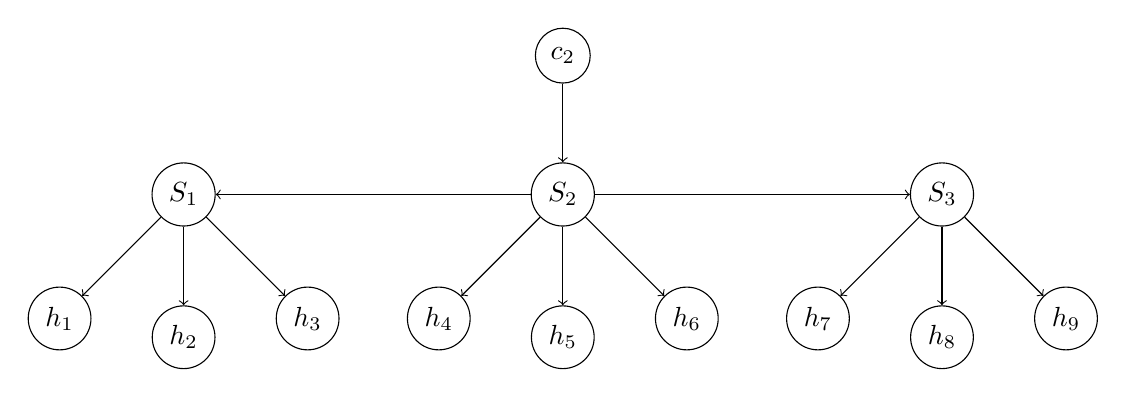
\begin{tikzpicture}[
      every node/.style={draw, circle},
      every on chain/.style={join},
      every join/.style={->}]

    {
      [start chain]
      \node [on chain] {$c_2$};
      \node [on chain=going below] {$S_2$};

      {
        [start branch=s1]
        \node [on chain=going left, node distance=4cm] {$S_1$};

        { [start branch]; \node [on chain=going below left]  {$h_1$}; }
        { [start branch]; \node [on chain=going below]       {$h_2$}; }
        { [start branch]; \node [on chain=going below right] {$h_3$}; }
      }

      {
        [start branch=s3]
        \node [on chain=going right, node distance=4cm] {$S_3$};

        { [start branch=h1]; \node [on chain=going below left]  {$h_7$}; }
        { [start branch=h2]; \node [on chain=going below]       {$h_8$}; }
        { [start branch=h3]; \node [on chain=going below right] {$h_9$}; }
      }

      { [start branch]; \node [on chain=going below left]  {$h_4$}; }
      { [start branch]; \node [on chain=going below]       {$h_5$}; }
      { [start branch]; \node [on chain=going below right] {$h_6$}; }

    }

  \end{tikzpicture}
  \caption{How a client message is forwarded to all end-hosts.}
  \label{figure:flow.client.forwarding}
\end{figure}
\todo{Få pilene til ikke å gå helt inn i noder (stealth?), og flytt
  side-switcher litt nedenfor switch i midten for å illustrere tid.}

When the leader receives a client packet, it will initiate the Paxos
algorithm.  In our simplified version of Paxos, it will then send
\texttt{ACCEPT} messages to the other two switches.

These switches will then send out \texttt{LEARN}-messages.
When a switch has received a majority of \texttt{LEARN}s, it will proceed to
send the last fragment down to its hosts.  The hosts will then combine the
fragments and pass the packet to the application.

The applications will then process the packet and, optionally, send back a
reply.\todo{Skal vi se bort fra hvordan vi velger ut svar fra endesystemene
og sender svar til klienten? Eller skal vi bare legge inn flows sånn at
kun den som mottok opprinnelig pakke kan svare klienten?}

\begin{figure}
  \centering
  \scriptsize
  \begin{tikzpicture}[>=stealth,x=1.2cm,y=1.2cm]
    \stdset{exec box color=white!20}
    \initstd
    \process{/S1}{$S_1$}
    \process{/S2}{$S_2$}
    \process{/S3}{$S_3$}
    \process{/c1}{$c_1$}
    \process{/hosts}{\textit{hosts}}

    % Groups
    \def\sw{/S1,/S3}
    \def\allsw{/S1,/S2,/S3}

    % Incoming client request
    \msg{/c1}{/S2}{Request}{v}{Forward}
    \mcast{/S2}{\allsw}{Forward}{v}{Store $v$}

    % ACCEPT
    \mcast{/S1}{\allsw}{Accept}{n,v}{On accept}

    % LEARN
    \alltoall{\allsw}{LEARN}{n,v}{On majority}

    % To hosts
    \mrcast{\allsw}{/hosts}{Request}{v}{Execute}

    \drawtimelines
  \end{tikzpicture}
  \caption{A client $c_1$ sends a request to the system. The message is
    forwarded to and stored on all switches.  The leader $S_1$ then sends out
      \texttt{ACCEPT} to all Paxos nodes.  They send \texttt{LEARN}s to
      all other switches.  When a switch has received \texttt{LEARN}s from a
      majority of nodes, it will send the message down to its
      \textit{hosts}, which then execute the client packet.  Not shown here
      is how we ensure that the client only gets back \textit{one} reply
      from the end-hosts.}
  \label{flow:simple}
\end{figure}
\todo{Husk å bruke EN IP-adresse utad mot klientene.}
\todo{Legg inn flere illustrasjoner her, oppdater graf og caption}
\todo{Merk, vi sender ut pakken til alle.. her kunne vi sendt til hosts
  direkte med fragmentering.. men vi kunne også bare sendt den ut til leader
    fra S2 og S3, og så sender leader ut hele pakken.. men vet ikke om det
    er nødvendig.. er like greit å gjøre med én gang? (det er sånn en kan
        finne ut hva som er best med benchmarks faktisk, som en alternativ
        konfigurasjon... merk også at vi KAN faktisk få synk-problemer her,
        så kanskje den BØR sendes til leder først for å få et offisielt
        pakkenummer????}

What we have accomplished here is using Paxos for
ordering\index{Paxos!ordering}\index{ordering} the client
requests down to the hosts, so that each host will receive packets in the
same order.  To test this, we will run simulations where several clients
send requests to the hosts. After some time, the state of each host should
be equal to each other.

\section{The Final Set of Flow Entries}
\label{chapter:final.flowtable}

\todo{oppdater dette}

\begin{table}[H]
  \centering
  \begin{tabular}{|l|l|}
    \hline \textbf{Match} & \textbf{Action} \\
    \hline From client & Fragment, store fragment 2 w/crnd, send fragment 1 to hosts \\
                       & Execute send-accept program \\
    \hline From host & Forward to client (TODO: Ignore, only allow one reply) \\
    \hline PAXOS JOIN  & Store MAC address and node id of switch \\
    \hline PAXOS LEARN & Execute program on-learn \\
    \hline
  \end{tabular}
  \caption{The final flow table for the Paxos leader.}
  \label{table:complete.match.leader}
\end{table}

\begin{table}[H]
  \centering
  \begin{tabular}{|l|l|}
    \hline \textbf{Match} & \textbf{Action} \\
    \hline From client & Fragment, store fragment 2 w/crnd, send fragment 1 to hosts \\
                       & Forward to leader \\
    \hline From host & Forward to client (TODO: Ignore, only allow one reply) \\
    \hline PAXOS JOIN from any & Store MAC address, node id and leader-flag \\
    \hline PAXOS LEARN from any & Execute program on-learn \\
    \hline PAXOS ACCEPT from leader & Execute program on-accept \\
    \hline
  \end{tabular}
  \caption{The final flow table for Paxos slaves.}
  \label{table:complete.match.slave}
\end{table}

\todo{Legg inn diagrammer for nettverksflyt, dette gjelder andre steder
  også.}

  \chapter{Analysis}

Here we will look at the performance profile of our various configurations.
Note that we are running everything on a software network simulator, and
therefore these performance tests will only be useful for giving us an
indication of \textit{relative} performances.

Therefore we will first need to establish a baseline for the system as it
is. We should then be able to compare various configurations against it.

\todo{Når ferdig, test med ekte software som MySQL, osv osv.}

For reference, the teste have been run on an Ubuntu GNU/Linux VM from the
Mininet site, loaded with our code and running in VirtualBox on a Mac OS X
laptop.

Instructions on how to run the tests are given in
\ref{chapter:appendix.benchmark}
\vpageref{chapter:appendix.benchmark}.

\section{Baseline --- ICMP ping on L2 learning switch using flow tables}
\label{chapter:baseline.benchmark}

The most basic setup we can test against is using our L2 learning switch
from chapter \ref{chapter:l2.learning.switch}
\vpageref{chapter:l2.learning.switch}.  This is fundamental to all our
configurations, because they all use it to make sure that packets are routed
correctly.

We will use the topology given in figure \ref{figure:baseline.topology}.

\begin{figure}
  \centering
  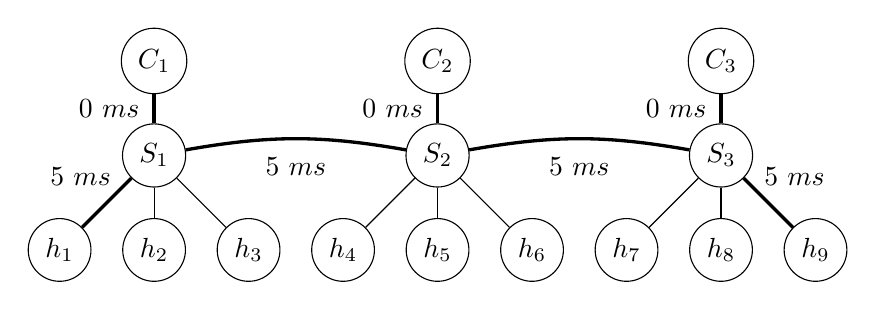
\begin{tikzpicture}[
    every node/.style={draw, circle},
    x=0.6cm,
    y=0.6cm]

    % Switches
    \foreach \n in {1,2,3} {
      \pgfmathsetmacro\x{(\n-2)*6}

      % Switch
      \node (S\n) at (\x ,  0) {$S_\n$};

      % Controller
      \node (C\n) at (\x ,  2) {$C_\n$};
      \draw (S\n) -- (C\n);

      % Hosts
      \foreach \h in {1,2,3} {
        \pgfmathsetmacro\pos{(\h - 2)*2}
        \pgfmathtruncatemacro\num{((\n - 1)*3) + int(\h)}

        % Host node
        \node (h\num) at (\x + \pos, -2) {$h_{\num}$};
        \draw (S\n) -- (h\num);
      }
    }

    % Switch links
    \draw (S1) to[out=10,in=170]
               node[below=-0.2cm, draw=none] {$5~ms$} (S2);

    \draw (S2) to[out=10,in=170]
               node[below=-0.2cm, draw=none] {$5~ms$} (S3);

    % Mark traversal path
    \draw [very thick] (h1) -- node[above left=-0.1cm,draw=none] {$5~ms$} (S1);
    \draw [very thick] (S1) -- node[left,draw=none] {$0~ms$} (C1);
    \draw [very thick] (S1) to[out=10,in=170] (S2);

    \draw [very thick] (S2) -- node[left,draw=none] {$0~ms$} (C2);
    \draw [very thick] (S2) to[out=10,in=170] (S3);

    \draw [very thick] (S3) -- node[left,draw=none] {$0~ms$} (C3);
    \draw [very thick] (S3) -- node[above right=-0.1cm,draw=none] {$5~ms$} (h9);
  \end{tikzpicture}
  \caption{Baseline topology with three switches $S$ and their controllers
    $C$.  The client $c_0$ will send ICMP ping packets to the farthest node
      $h_9$.  The packets will go through three links with a configured
      latency of $5~ms$.}
  \label{figure:baseline.topology}
\end{figure}

Before we present the results, let's look at what we should expect from the
configuration above.  The three links the packets need to cross each have
$5~ms$ latency.  There is some latency in each switch and in each end of the
link ($c_0$ and $h_9$) as well as between and in the switches and their
controllers.

In total, one would expect the \acf{RTT} to be
\begin{gather}
  RTT_{c_0, h_9} = 2\left( \sum L + \sum P_S + \sum P_C \right) + P_{c_0} + P_{h_9} + K
  \label{equation:baseline.rtt}
\end{gather}

That is, the one--way latencies for all links ($L_{h_1,S_1}$, etc.), processing time $P$ for
$S,~C,~c_0,~h_9$ and a constant $K$ for any extra noise on the network
(e.g., from the OS, virtual machine engine, when flushing file buffers for
 recording results and so on).
Equation \ref{equation:baseline.rtt} is inspired by \cite{DBLP:conf/cnsm/PhemiusB13}.
\todo{Refiner formel, den kan ha feil!}

For simplicity, we will set $P_{c_0},~P_{h_9}$ and the
latencies for links between switches and controllers to zero.\footnote{When
flow table entries are installed, one should see very little traffic going
to the controllers, meaning that we can
assume that $L_{C,S} \to 0$ when the flow tables have been ramped up.
There will still be some background noise on the network, though, and we
print the ones we don't have rules for as dots in the controller log.}
We have also removed the fall--back link
between $S_1$ and $S_3$ seen in figure \ref{figure:graph.three.switches}
to make sure that ICMP packets won't take different paths on the network.
We could attempt to measure $K$ by running Mininet with two nodes linked
with zero bandwidth, but we will simply set it to zero as well.

Filling in the known values gives
\begin{gather}
  RTT_{c_0,h_9} = 40~ms + 2\left( \sum P_S + \sum P_C \right)
  \\
  RTT_{c_0,h_9} = 40~ms + 2L~\text{where}~L = \sum P_S + \sum P_C
  \label{equation:expected.baseline.rtt}
\end{gather}

We will now use the \texttt{ping} command to send out many packets per
second.  The controller will install flow tables with idle and hard timeout
set to one hour. The flows we install (flow table entries) will match on
Ethernet packets whose destination addresses are on known ports.

Table \ref{table:baseline.summary} gives a summary and figure
\ref{benchmark:l2.learning.switch.ping} shows the plots.

% Table with summary of RTTs (mean, median, etc.)
\input{data/pings-summary.tex}

\begin{figure}
  \centering
  \includegraphics[width=\textwidth]{data/pings.pdf}
  \caption{\acs{RTT} for ICMP PING on the L2 learning switch using flow tables.
           We can clearly see the ramp--up time for the controller as it
           adds flow table entries to have the switch automatically forward
           Ethernet packets. The plot shows the \textit{median} value in red
  and the \textit{mean} in gray.  Because of the ramp--up phase, the mean is a poor
  indicator for the values after warm--up.  As we have a relatively large
  number of samples, the median gives a more realistic picture of the
  situation.  This can clearly be seen in the plot.}
  \label{benchmark:l2.learning.switch.ping}
\end{figure}

There is a noticeable ramp--up time before flow tables get entries, and
because of this we will have some variation in the samples. Therefore we
would assume to get a mean value larger than the median.  Looking at the
histogram, this seem to be the case, and therefore the median should give a
more realistic value for the RTT when the system has settled down.

Other than that, we see that the median is in line with our
expectations---the RTT is clearly bound an RTT of 40 ms.  We can now insert
the median value in equation \ref{equation:expected.baseline.rtt}.

\input{data/pings-results.tex}

If we run the test again \textit{without} installing flows, we should see
all the processing being moved over to the controllers.  This should let us
give an estimate for $P_C$.

We ran the test again  with the only difference being that we don't
install flows.  The summary can be found in table
\ref{table:baseline.noflows.summary} and the plots in figure
\ref{figure:baseline.noflows.plots}.

Using the estimated value for $P_C$, we see that

\begin{gather*}
  L = 3P_S + \sum P_C = 1.60~ms \\
  \sum P_C = 3P_C = \frac{75.80~ms - 40~ms}{2} = 17.90~ms \\
  P_C \approx 5.97~ms
\end{gather*}
\todo{Put this part in an R script}

When all the work is being done by the controllers, their individual
one--way processing latency is around $5.97~ms$.  The ramp--up this time
refers to the fact that the controllers still need to populate their
MAC--to--port tables so they can forward packets instead of broadcasting
them.  There is also a spike in RTT at the very end.  We haven't looked more
into this.
\todo{Er en spike imot slutten også, hvorfor? Er det buffer-skriving?
  Isåfall, da burde den også være på forrige graf... hva skjer?
Og hvorfor er det så konsistent?}

\input{data/pings-noflows-summary.tex}

\begin{figure}
  \centering
  \includegraphics[width=\textwidth]{data/pings-noflows.pdf}
  \caption{Rerun of baseline benchmark
    (ch.~\ref{chapter:baseline.benchmark}), but without installing flows.
  Medians are shown in red and means in gray.}
  \label{figure:baseline.noflows.plots}
\end{figure}

\todo{Remove outliers and show numbers.}
\todo{Bruk boxplot() i R når en skal sammenligne. Og hiv inn tall i tabell
  for sammenligning sammen med plot. Plot trenger ikke være gigantisk stor.}

To sum up this benchmark, we have plotted both values in figure
\ref{figure:baseline.combined.plot}.

\begin{figure}
  \centering
  \includegraphics[width=\textwidth]{data/pings-combined.pdf}
  \caption{RTTs for baseline test with and without using the flow tables.
  Medians are shown in red and means in gray.}
  \label{figure:baseline.combined.plot}
\end{figure}

\section{L2 learning switch, key--value store}
\label{chapter:benchmark.l2.kv.noflows}

First we need a baseline.  Here we have a topology of two switches $S_0$ and
$S_1$ with a controller each.  The switches has three hosts, $h_0, \dots, h_5$.
A client $c_0$ is connected to $S_0$. We're running Python
key--value--stores on each host, and $c_0$ will issue a get--request
followed by a put--request to the host $h_5$, which is connected to $S_1$.
We measure the time for each request, divide it
by two and call it latency.\footnote{We basically assume that the packets
take an equal amount of time back and forth, and divide by two to get this
time.}

There are two controllers $C_0$ and $C_1$ for the switches $S_0$ and $S_1$,
respectively.  In this situation, the packets from $c_0$ need to travel
over two switches.

The network is running on Mininet, a software network simulator, on a Linux
virtual machine running on an Mac OS X box.  All the links in Mininet have
been set up with $10 Mbit/s$ bandwidth, $5~ms$ latency and no packet
loss.  These links have been set up with \ac{HTB}
\cite{devera2002hierarchical} enabled, which Open vSwitch\index{Open vSwitch}
 uses for providing rate limiting.

In this first benchmark, the switches will send each packet up to the
controllers.  The controllers implement L2 learning switches and will not
install any flow table entries for rapid dispatch.

On the x--axis is the time in seconds.  On the y--axis is the latency for
get and put requests.

The result can be seen in figure \ref{benchmark:l2.learning.switch.no.flows} 
\vpageref{benchmark:l2.learning.switch.no.flows}.

What is surprising here is that the put--requests have much higher latency
than the get--requests. We don't know why this is.\todo{Finn ut! Er det pga
  pakkene er større? Eller andre grunner?}

\section{L2 learning switch, key--value store, flow entries}

We have the same setup as above, but this time we install flow entries that
will automatically forward the packets.  The flow table entries will match
on as many fields in the packets as possible.

The flow table entries have idle and hard timeouts set to 10 seconds.
In other words, we should be able to see some increased latency every ten
seconds.

% Present both plots together
\begin{figure}
  \centering
  \begin{subfigure}{\textwidth}
    \centering
    \includegraphics[width=\textwidth]{data/data2.eps}
    \caption{L2 learning switch without using flow tables.}
    \label{benchmark:l2.learning.switch.no.flows}
  \end{subfigure}

  \centering
  \begin{subfigure}{\textwidth}
    \centering
    \includegraphics[width=\textwidth]{data/data3.eps}
    \caption{L2 learning switch using flow tables.}
    \label{benchmark:l2.learning.switch.with.flows}
  \end{subfigure}
\end{figure}

The result can be seen in figure \ref{benchmark:l2.learning.switch.with.flows}
\vpageref{benchmark:l2.learning.switch.with.flows}.

Here we can see that the latency has been reduced somewhat.\todo{Hvor mye?
Hva med å plotte over hverandre, hva med å lage average eller root mean
square eller noe sånn?}

We also see some latency spikes around every ten seconds, as expected.

\todo{Plott med flere verdier, istedenfor å vise seconds på x--aksen kan vi
  vise elapsed time, som i at den starter på 0 sekunder.}

These two benchmarks will serve as a baseline to which we will compare our
performance when we enable Paxos on the switches.

Remember that when we run Paxos, we will still have to use the L2 learning
switch for the nodes to be able to communicate.

\todo{Trendlinjner, moving average, fitting osv... må ha det i grafene, må
  også ha litt statistisk analyse av tallene selv osv.}

\section{Three switches, Paxos on controller}

\todo{Få data}

\section{Three switches, Paxos on controller and flow table}

\todo{Få data}

\section{Other solutions}

We chose to use OpenFlow as the basis for our system.
We could just as well have used a networking system that already supported
programmability in some way, for instance the Intel DPDK\todo{Needs
citation}.\todo{Also needs defense.}

\todo{Flytt evt dette ned til improvements--delen}

  \chapter{Improvements and future work}

Here we will discuss improvements that could have been made to our system
but was out of scope.

\section{Monitoring link-status}

OpenFlow makes it possible for controllers to receive notifications when
link-status\index{link-status} changes.  In OpenFlow 1.0, this is restricted
to receiving \textit{link up} and \textit{link down}
notifications\index{OpenFlow!link-status}.

We could take advantage by monitoring the links to other switches.
If the leader goes down, leader-election should be performed.
If any switch goes down, then hosts should synchronize their state with
other hosts (and the same if a single host goes down).

\section{Leader-election}

Our system does not implement
leader-election\index{leader-election}\index{Paxos!leader-election} at all.
This should be part of any complete Paxos system.

It would be easy to add more Paxos message types to our tables, and the
algorithms could be implemented as small bytecode programs.

\section{Using IP-fragmentation for buffering}

For the system to perform well, we don't want to store client packets in the
switch or the controller.  Instead, it would be nice if we could just pass
along client packets directly down to the end-hosts.\index{buffering}

However, this means that the hosts will process the packets before we have a
chance to perform Paxos ordering.

We propose a neat solution to this problem.  When a switch receives a client
message, it will immediately perform IP-fragmentation\index{fragmentation} of the message and
send the first fragment to the hosts.  The hosts networking stack will then
buffer the packet and wait for the last fragment.

When the Paxos consensus algorithm terminates, we will send the last
fragment down to the host, which will then pass the packet up the stack to
the server program.

We still need to store fragments, but if we choose the fragmentation offset
wisely, we need only store very small fragments.

The downside to this is that we break MTU rules, and some systems may behave
strange---or not at all.  But for our purposes we think this is a good
solution.

For this we need some new OpenFlow actions for fragmenting packets, storing
them and then forwarding the stored remaining fragment.

\section{Full Paxos support}

The most obvious improvement to this project would be to implement all of
Paxos: Trust\index{Paxos!trust}, prepare\index{Paxos!prepare} and
promise-messages\index{Paxos!promise} and what has been mentioned above.

However, we stated in the introduction that we wanted to constrain ourselves
to just look at how we could implement accept and learn-messages, as a
proof of concept.

Our solution would actually make it quite simple to add support for the full
Paxos algorithm.  Furthermore, our solution is very \textit{modular}, in the
sense that the controller can select which programs to compile to bytecode
and install on the switch.  This means we could have several different
leader election algorithms as small, self-contained programs, and select
which one to use for a given system.

The flow table rules are also extremely flexible as they are, and allows for
small, but easy, optimization opportunities (for instance, to support a new
Paxos message type only requires one new flow table entry and one new
program).

\todo{Flytt deler av dette ned til konklusjon, for det er et ganske sterkt
argument dette med modularisering og at det lett kan bygges videre på!}

\section{Security}

A networking thesis like this would not be complete without a brief
discussion of security concerns\index{security}.

Basically, we have ignored all aspects of security.  While OpenFlow
communicates over a secure channel using \ac{TLS}\index{OpenFlow!TLS}, we
allow bytecode to run on the switches themselves.  Naturally, we should have
chosen a bytecode \acs{VM} that allows for \textit{sandboxed execution}.
I.e.,~it should not be able to access any other facilities than pure
programming constructs and the restricted interface to the switch
capabilities.

\todo{Tenk mere og skriv mere}

\section{Related work}

\todo{Skriv om andre prosjekter, er bla en load balancer skrevet for
  openflow og se på corfu-paper. Bør dette underkapittelet flyttes til
    introduksjon eller tidlig i oppgaven? Vet ikke hva som er vanlig
    struktur}

\section{Other platforms}

Look at other programmable networks.

Openflow 2.0\index{OpenFlow!version 2.0} is rumoured to have an experimentation api, but the stuff in
this thesis is actually far ahead of that, more flexible.
It would actually allow one to experiment with what should be part of
OpenFlow 2.0.

  \chapter{Conclusion}
\label{chapter:conclusion}

\todo{Vis at vi har nådd målene våre, vis svakheter, vis benchmark, osv. Bør
  være en ganske kort oppsummering (max en side).}

\todo{Ta med at vi har sett vekk fra security, feks utnytting av
  algoritmene og sånt}


  % Bibliography should come before appendix
  %
  % Add unused citations here to make them appear in the bibliography.
  % A wildcard prints out all references.
  %\nocite{*}
  %
  % These must be on ONE line without spaces
  \bibliography{bibliography/mininet,bibliography/networking,bibliography/openflow,bibliography/paxos,bibliography/sdn,bibliography/software,bibliography/source-code,bibliography/books}
  \bibliographystyle{plain}

  \appendix
    \chapter{Running the thesis code}
\label{chapter:install.vm}

The best way to run the thesis code is to download a virtual machine image.
We used VirtualBox\index{VirtualBox} for running this image, but it should
also work on VMWare\index{VMWare}.  It comes preloaded with
Mininet\index{Mininet}, Open vSwitch\index{Open vSwitch},
  POX\index{POX}\index{controller|seealso{POX}},
  Wireshark\index{Wireshark} and more.

The user \texttt{mininet} has password \texttt{mininet} and has
\texttt{sudo}-rights.

\section{Downloading and verifying the VM image}

The Linux\index{Linux} VM image containing a ready-to-run version of the
code in this thesis, along with all its tools, can be downloaded from

\begin{center}
  \url{http://csl.name/thesis/mininet-vm-x86_64.vmdk}
  \label{gpg:url}
\end{center}

To verify that this image has not been modified after the time of thesis
submission, you should download the author's GPG-key\index{GPG} (listing
\ref{gpg:key}, p.~\pageref{gpg:key}) and use it to verify the file digest
in (listing \ref{gpg:signature}, p.~\pageref{gpg:signature}).

To import the author's key, you can use \ac{GPG} or any software compatible
with PGP\index{PGP}.  Importing the key is done by running the command
\texttt{gpg --import} and pasting a copy of the author's key, ending the
input by hitting \texttt{CTRL+D}.\footnote{You can also copy the key to a
  file \texttt{key.asc} and importing it with \texttt{gpg --import key.asc}}
%
\begin{Verbatim}
$ gpg --import
# paste in author's key and hit CTRL+D
\end{Verbatim}
%
You should now see they key on your key-ring.
%
\begin{Verbatim}
$ gpg --list-keys
\end{Verbatim}
%
The key's fingerprint should be the same as below:
%
\begin{lstlisting}[label={gpg:key.fingerprint}]
pub   4096R/FA475DD2 2013-04-23 [expires: 2016-04-22]
      Key fingerprint = D611 0F24 4813 9908 1CFE  79BA 1AB4 2C77 FA47 5DD2
uid                  Christian Stigen Larsen (General key) <csl@csl.name>
sub   4096R/D2495ED9 2013-04-23 [expires: 2016-04-22]
\end{lstlisting}

Finally, you need copy the VM image digest (listing \ref{gpg:signature}
\vpageref{gpg:signature}) to a file called
\texttt{mininet-vm-x86\_{}64.vmdk.asc}, placed in the same directory as the
downloaded VM image \texttt{mininet-vm-x86\_{}64.vmdk} (from \vref{gpg.url}).
You can then run \texttt{gpg --verify mininet-vm-x86\_{}64.vmdk.asc} to verify
the digest against the author's key.\footnote{Note that if you haven't
marked the author's key as \textit{trusted}, you will get a warning about
it.  But it should say that the signature is good.}

\begin{Verbatim}
$ gpg --verify mininet-vm-x86_64.vmdk.asc
gpg: Signature made Thu Apr 24 11:52:02 2014 CEST using RSA key ID FA475DD2
gpg: Good signature from "Christian Stigen Larsen (General key) <csl@csl.name>"
\end{Verbatim}

\lstinputlisting[
  caption={GPG signature for the thesis VM image.},
  label={gpg:signature}]{mininet-vm-x86_64.vmdk.asc}

% This text is long and must be on its own page
\begin{lstlisting}[
  float,
  caption={The author's public GPG-key},
  label={gpg:key}]
-----BEGIN PGP PUBLIC KEY BLOCK-----
Version: GnuPG v1

mQINBFF21LABEACrXyM2pQ9rl0TFlubOUBb9OtUF+wxCIqFCCvgVoYNCbldXMixc
wJzv6y76m/xfrpzZjl73tAnbY3WezHpY5MtPc/OtaW0BL5nlx1i21tfoW4YpHF4N
jPXkLYFiglb43eChRE5xbH14iaJ335SLt4YKFMIArug6g9tBjyjkXvvZNXJOKxDr
jUFX13hIKzyF2x298j+sNwlXy8SUB1NM6NNrtmhD46QMqlxBn2/+U1gXQrDpBxJR
PlXomaiTNb9hEH2XQcTfPMnFbZTzGO2fWA/njzSRC3L5gwsbGronFbnkf0rN8RrF
amPOu171NsH5YhHbsVpGG6KepGA/i1zq9sPXXYHKC0NdOHdrGhEuOjDNWOy/hu0n
eldUclSmnL04QHIwGkZomrgyQT2GcNM0U5wyXZ4QHKjamNoT0etLpXPmXGMQhSVY
psVvchQfBzzohuiOqtb3KdbAqua09FB86AfmWOXsHnvv3A7q864QllpPhP0SwpZ/
bW9e/2POWYpaEZ1jWLkhj1ctnRDBP+2lvKu0zp8wvN4xRDVCPxHonbKhrWV0vCD7
UP+PAvqfhlgorXSeaSZvhMa4evSrYxZwYj52m3x3P5dSFDeFZFgrbJ/fNyRJRino
8dTYT/+ccEj1y+mGDPV2T0A60c+ZHmhpg1cshtOXk+c0qCfYEndmSAQT7QARAQAB
tDRDaHJpc3RpYW4gU3RpZ2VuIExhcnNlbiAoR2VuZXJhbCBrZXkpIDxjc2xAY3Ns
Lm5hbWU+iQI+BBMBAgAoBQJRdtSwAhsDBQkFo5qABgsJCAcDAgYVCAIJCgsEFgID
AQIeAQIXgAAKCRAatCx3+kdd0p8aD/9a6MBhfkanB4vZCKhNYjM89Oxo/E06zEAm
KCxy3N2TnRBkqwQFkflKVJe9nw2PsSITBbKDIVWV3jJ06Lgx+hVMyu5srvCPirSv
dF/0chS0tNL52ZIz13EJnprZZg80+CYPQoHPgOnS8xg+qV1bROFB5n4K+cyCy4Db
l36k316zZ042NwoaEMHqgLd7Lr55FpNyoHaGtGOLSmW4BQkfldx6G1kdJefFY43h
bj2YICuj6vY8ztmPVjrmtoiomMFAj+dIWW+z1TAsQ4lUhWpXEEIW5lNePBce2jVZ
1d+oWe9u//RzBRBKy/jI0GxE+Pq3ZdLOxM87tejYDcdb/QUQSGmQ4QugxvKXol5W
XT8wsfNm+c2amolnpVuWHMCHHZSY8PGLJwBc+oZOlEBrXxE8dU8uD3A3fBQgiABD
ETLEs0KzS9oo1m6EGrZSD0v3cbR4XtrEw9elUIhS6mwUpjoFqanNgwUXJiomsvjR
63FOw1wzO7TMz8weRr+ZUXMwvg7QEuxkIhGqnaAk5t1BMKNFneKs7NApwa2FyZ6q
oVZXG6INEee8Uw+SBph9jq9O2mBueiWVNei7+tHcZgqZAmNyPh1cwo37c4yHX707
hqzmdnnW54/HPDeIly4gC/wRQZUkWb5z981XiJgSLzppKdCyiX4ygJ730WdBjjYq
QW8ZING9xrkCDQRRdtSwARAA6xNB6yQIhYUkIZ1UfBq91iQIFrt6v0cxCUqCqFYG
y5+bnqOIoZqvNOW0oMPWKYNaCGow+lPFz8+alFBrrNzznoHYTQwNC68qaXxoIMH4
o4Ah+IK5KQ9g/iUu9fbCPcpFYH90z4TJM2uAeZO9eJQmQqaWqfj2Y9IFDNEgDEln
rq0BgpD1R+qArPsGT0i34wTQ+cO9apGZB8FH7bGqvqReBmifW9vHh7DVtA+og9Js
wWNJAaRCHv/AXnqfRxwCoeFQQGW4cncDDuaYvC6ADPPvQ9c6FzaFE36p45OKPzy/
Z1gAjDhs9dlkdtYxKj8uyMDBlDaC4J/rPfZ7kD2PFi0iXfEk0JyAXihaAjz3eJaH
xwnjRQVNrP4PW+3We3DI15VzgDmzjem2rVHBVigNhi5dFNbhSmTThQx2wRlOI57s
D3QDvJl+ppPHlP0yQETe4F9Op6diLm7jXHmvezII5RN29gKjgnz0jvXBKqHfXIco
SgB418Jp+XTzsuA/SuhuiOo/d0ac/RiM95pu8upYLbRo1VqJwQyTPqUzj0zWiSTl
waekJpwwkQONZwFtquYYVdLhR30X1GX92OfAd9JdbMGK7WR3RZfwNSUWKnCSbqoi
WAjHW9sEK7ltU8TKKXJjbseSPNKk9Khc8h87skmNofOknY03nTG50YTvHSWpxxdL
feEAEQEAAYkCJQQYAQIADwUCUXbUsAIbDAUJBaOagAAKCRAatCx3+kdd0npOEACU
Kw4AR5GBjBTcrb0JQj+YFBZO4heYA/4UMcbPqvwJzeX0nSuZ+vkB9GV08nd7/jC2
+CiHlTlrtoH40S7SdOGoZgNx7WHeHFKLo8i29lUf0ID55TOs0EctYwX/MWLWt8JJ
uZ8OXQnrXL9Mtg1yybkftMiqSmAYtWfcX6Wv86zpPzM8K4kWkd5o3NNFWBareEqL
fmdjNyyumpYX+5tHMc2v7oxG/oEC5SCVJmF5ZzFuiBBvJPPIxfYHajoR1Xz+kKf/
RDtbTJxnR0Ftfhwb5Tv4iX6rYXHwvC6bhKB4Knndba+WeN7tYKAX7rLEasdzubGj
vSZgJD3CZykk7WIq5exDHTw5E4BtgOZc5LxOf2KsWBxks6vdjbeAICA135tKxtDB
lPMytrCMNy6JNoA0fFB/KxSnOhOIxH4Ar/vXaBJxI0mQuhs9Qt+27alf6R6OgjIN
S7KQ5l3MaUFUaiRwvGJeeolT+e6X/ssLZQyWDkrNxkonZ+GhbSO5p5zgGXA3PXGg
X/18vQyTCn1jt+jzr+f/6BW+E9pqusJ4MYdDM5ThKv7TjyslMW71cdFjCHNkf1/k
9zduikQwVddgU4Ha3T6+jOY0VLncguA7UnMTOdFGdL4SchZjswDzOHPcOxC4+Un5
x7JoKcugqMAINWCfPKu5IXU6SqSkKA6ddVG/SJ5wcA==
=iAwm
-----END PGP PUBLIC KEY BLOCK-----
\end{lstlisting}
\clearpage % Clear page after this key as it's pretty long.

\section{Setting up the VM image}

The author's settings in \textit{VirtualBox}\index{VirtualBox|seealso{VM}}
for the Linux VM\index{VM!setting up} are given in table
\vref{table:vm.settings}.  The fields marked as \textit{needed} must be set
as shown, otherwise the VM may not work properly.

Start VirtualBox and create a new VM.  Then point to the provided VM image
(the option \textit{Use an existing virtual hard drive file})
and copy the settings in table \vref{table:vm.settings}.

When you boot the VM, you should try to ping a remote host on the internet,
then you should attempt to \texttt{ssh} into it from a terminal on the host
computer.

% TODO: Fix the VERTICAL spacing as well, it is still white
\begin{table}[ht]
  \begin{tabular}{!{\vrule width -1pt}c
                  !{\vrule width -1pt}l
                  !{\vrule width -1pt}l}
  \hline
    \textbf{Needed}    & \textbf{Field}       & \textbf{Value} \\
    \hline
                       & Name                 & mininet \\
\rowcolor{verylight} * & Operating system     & Ubuntu (64 bit) \\
                       & Base memory          & 1024 MB \\
\rowcolor{verylight} * & Boot order           & Hard disk \\
                       & Acceleration         & VT-x/AMD-V, Nested Paging \\
                       & Display Video memory & 16 Mb \\
                       & IDE Secondary Master & vboxguestadditions.iso \\
                       &                      & CD/DVD \\
\rowcolor{verylight} * & SATA Port 0          & \texttt{mininet-vm-x86\_{}64.vmdk} \\
\rowcolor{verylight} * &                      & Normal, 8,00 GB \\
\rowcolor{verylight} * & Network Adapter 1    & Intel PRO/1000 MT Desktop \\
\rowcolor{verylight} * &                      & NAT \\
\rowcolor{verylight} * &                      & MAC: \texttt{FEEDFACEBEEF} \\
\rowcolor{verylight} * & Network Adapter 2    & Intel PRO/1000 MT Desktop \\
\rowcolor{verylight} * &                      & Host-only Adapter, 'vboxnet0' \\
\rowcolor{verylight} * &                      & MAC: \texttt{0800270A8160} \\
    \hline
  \end{tabular}
  \caption{Author's settings for the VM image.}
  \label{table:vm.settings}
\end{table}
\index{VirtualBox|seealso{VM}}
\index{VM!VirtualBox settings}

It is important that you set up the network
\textit{exactly} as shown, otherwise it may not function correctly.\footnote{
  If it stil does not work, make sure you have set up the guest OS
    networking settings correctly (ch.~\vref{chapter:guest.settings}).
  You may also want to edit the file
  \texttt{/etc/udev/rules.d/70-persistent-net-rules}.
  Update the corresponding MAC address and comment out all other lines, then
  reboot the VM.
   You may also need to change the VM's IP-address in
  ch.~\vref{chapter:ssh.setup}. If unsure of the IP-address, type
  \texttt{ifconfig eth1 | grep inet} to see the VM's address.
}

The \texttt{vboxguestadditions.iso} is not needed. We have used it only to
enable sharing of folders between the VM and host computer.

Remember that you can log in using the user \texttt{mininet} with the
password \texttt{mininet}.  This user should be able to get a root shell by
typing \texttt{sudo bash}.

\subsection{Guest OS network settings}
\label{chapter:guest.settings}

To be able to use \acs{NAT} on your VM, you need to set it up on your guest
OS networking settings in VirtualBox.

In the VirtualBox manager, go to preferences, network, \textit{NAT Networks}
and add a \acs{NAT}-network called \textit{NatNetworking}. Use the settings
from table \vref{table:natnetworking.settings}.

You also need to add an entry under the tab \textit{Host-only Networks}
using the settings in table \vref{table:hostonlynetworks.settings}.

\begin{table}[H]
  \centering
  \begin{tabular}{ll}
    \hline \textbf{Field} & \textbf{Value} \\
    \hline
      Enable network & Yes \\
      Network name & NatNetwork \\
      Network CIDR & 10.0.2.0/24 \\
      Supports DHCP & Yes \\
    \hline
  \end{tabular}
  \caption{Settings for guest OS NAT networking.}
  \label{table:natnetworking.settings}
\end{table}
\index{VM!network settings}

\begin{table}[H]
  \centering
  \begin{tabular}{ll}
    \hline \textbf{Field} & \textbf{Value} \\
    \hline
      \textbf{Adapter} & \\
      Name & vboxnet0 \\
      IPv4 address & 192.168.56.1 \\
      IPv4 network mask & 255.255.255.0 \\
       & \\
      \textbf{DHCP server} & \\
      Enable server & Yes \\
      Server address & 192.168.56.100 \\
      Server mask & 255.255.255.0 \\
      Lower address bound & 192.168.56.101 \\
      Upper address bound & 192.168.56.254 \\
    \hline
  \end{tabular}
  \caption{Settings for guest OS Host-only Networks.}
  \label{table:hostonlynetworks.settings}
\end{table}
\index{VM!network settings}

\subsection{Setting up SSH}
\label{chapter:ssh.setup}

In order to work with the VM, you need to add the following optios to your
local \texttt{\~{}/.ssh/config}.

\begin{verbatim}
Host mininet
  Hostname 192.168.56.102
  User mininet
  ForwardX11 yes
  ForwardAgent yes
  RequestTTY yes
\end{verbatim}
\index{VM!ssh}

X11-forwarding\index{VM!X11 forwarding} is required in case you want to start xterms on Mininet
nodes or run Wireshark.\index{VM!Wireshark}  Note that it also forwards your
ssh-agent---you may not strictly need this.  The \texttt{RequestTTY}-option
is \textbf{very important}, because it lets us start terminal programs on the remote
host. Without it, some of the examples here will leave processes running in
the background on the remote host when you SIGINT them (CTRL+D).\footnote{If
you don't use this option, you can manually type \texttt{ssh -t} to request
TTYs correctly.}

You may need to change the \texttt{Hostname}-parameter for your particular
system.  Doing this correctly saves you time when the host computer changes
networks.

To be able to logon passwordless, you need to upload your public key:

\begin{verbatim}
$ cat ~/.ssh/id_rsa.pub | ssh mininet "cat - >> ~/.ssh/authorized_keys"
\end{verbatim}
\index{VM!ssh}

Boot the VM and make sure you can log on to it without typing a password:

\begin{verbatim}
$ ssh mininet
\end{verbatim}

\section{The thesis source code}

You can find the thesis source code on the Mininet VM under
\texttt{\~{}/bach}.

\section{Running the thesis code}

To start the first example...
\todo{Write instructions on how to run the thesis code here.}

\section{Building code}
\label{chapter:compiling}

\subsection{Open vSwitch}
\label{chapter:compiling.ovs}

To build Open vSwitch\index{compiling|seealso{Open vSwitch}}\index{Open
vSwitch!building} on the VM, do the following:

\begin{Verbatim}
# Remove the preinstalled ovs
$ sudo apt-get remove \
    openvswitch-common openvswitch-datapath-dkms
    openvswitch-controller openvswitch-pki openvswitch-switch

$ cd ~/ovs
$ ./boot.sh
$ ./configure --prefix=/usr \
              --with-linux=/lib/modules/`uname -r`/build

# To compile ovs
$ make
$ make test # optional; takes some time

# To install
$ sudo make install
$ sudo make modules_install
$ sudo rmmod openvswitch
$ sudo depmod -a

# Now restart Open vSwitch
$ sudo /etc/init.d/openvswitch-controller stop
$ sudo /etc/init.d/openvswitch-switch stop

# Disable start of controller on boot
$ sudo update-rc.d openvswitch-controller disable

# And start again
$ sudo /etc/init.d/openvswitch-switch start

# Check that it's running
$ ps auxwww | grep openvswitch

# The executable ovs-controller changed name to test-controller
# in a recent ovs version, and Mininet relies on it:
$ sudo cp tests/test-controller /usr/bin/ovs-controller

# Check the version
$ sudo ovs-vsctl show
cd702e96-d4af-4803-9e2f-ecc2f7abcd6a
    ovs_version: "2.1.0"

$ modinfo openvswitch
filename: /lib/modules/3.8.0-35-generic/kernel/net/openvswitch/openvswitch.ko
license:        GPL
description:    Open vSwitch switching datapath
srcversion:     15C32AD9E04F379CAC3D68E
depends:
intree:         Y
vermagic:       3.8.0-35-generic SMP mod_unload modversions
\end{Verbatim}

\subsection{POX}

\todo{hvordan kompilere pox}

\subsection{Thesis code}

The thesis code is mostly written in Python, so no steps are necessary.
The only thing to remember is to use the correct PYTHONPATH.  You are
recommended to use the makefiles for this. We have also added symlinks where
needed, so you should not need to worry about it.

\todo{Hvordan bygge koden vår, C-koden, osv.}

\section{Running the benchmarks}
\label{chapter:appendix.benchmark}

To run the benchmarks yourself, you first need to set up the Linux VM image
by following the instructions in \ref{chapter:install.vm}
\vpageref{chapter:install.vm}.

You absolutely need to have set up \texttt{ssh} as shown in
\ref{chapter:ssh.setup} \vpageref{chapter:ssh.setup}, because we need
correct allocations of TTYs.

When you have done that, you may want to restart your Mininet before running
benchmarks.  This is to make sure that no processes from previous runs are
hanging in the background.\footnote{There may even be hanging processes from
the time the VM image was uploaded.} The test code mostly takes care of
this, but to be on the safe side, reboot with

\begin{Verbatim}
$ ssh mininet
$ sudo shutdown -r now
\end{Verbatim}

\subsection{Baseline benchmark}
\label{chapter:appendix.baseline.benchmark}

To run this benchmark\index{benchmark}, run the following on your local computer

\begin{Verbatim}
$ ssh mininet make bench-baseline
$ ssh mininet make bench-baseline-noflows
\end{Verbatim}

If you prefer to run Mininet and the controller in separate terminals, you
can start each one independently:

\begin{Verbatim}
# Terminal 1 (start first)
$ ssh mininet make bench-baseline-pox

# Terminal 2 (start after POX is up)
$ ssh mininet make bench-baseline-mininet
\end{Verbatim}

After the test runs complete, there are two result files that you can
download locally:

\begin{Verbatim}
$ scp mininet:~/pings.txt mininet:~/pings-noflows.txt .
\end{Verbatim}


  % Because of hyperref/makeidx/toc bug, we have to insert anchors
  % ourselves here.  See
  % http://tex.stackexchange.com/questions/138903/wrong-hyperref-for-index-in-tableofcontents-since-texlive-2010
  %
  \clearpage % may not be needed with imakeidx
  \phantomsection % may not be needed with imakeidx
  % Also add to ToC
  \addcontentsline{toc}{chapter}{Index}
  \printindex
  \chapter*{Colophon}
\label{chapter:colophon}

This thesis was typeset using \LaTeX{} from the \TeX{}
\textit{Live}-distribution on a Mac OS X along with several packages.

The figures were made using \textit{TikZ}.
Statistical calculations and plotting were made using \textit{R}.

\end{document}
